\documentclass{article}

\usepackage[utf8]{inputenc}
\usepackage{a4wide}
\usepackage{graphicx}
\usepackage{amsmath}
\usepackage{amssymb}
\usepackage{amsfonts}
\usepackage{amsthm}
\usepackage{wrapfig}
\usepackage{makecell}
\usepackage{xspace}
\usepackage{caption}
\usepackage{wrapfig}
\usepackage{float}
\usepackage{MnSymbol}
\usepackage{todonotes}
\usepackage{parskip}
\usepackage{chngpage}
\usepackage{multirow}

\newcommand{\patrick}[1]{\todo[color=purple!25!white]{Patrick: #1}\xspace}

\newtheorem{condition}{Condition}
\newtheorem{conjecture}{Conjecture}
\newtheorem{observation}{Observation}
\newtheorem{lemma}{Lemma}
\newtheorem{corollary}{Corollary}
\newtheorem{definition}{Definition}

\newcommand{\etal}{et.al\xspace}

\def\polylog{\operatorname{polylog}}

\title{Stochastic Monkeys}
\author{}
\date{}

\begin{document}

\maketitle

\section{Summary of Results}

\begin{tabular}{|c|c|c|c|c|c|}
    \hline
     & & 2 D & 1 M, 1 D& 2 M & $O(n^2 \polylog n)$ Preprocessing \\
     \hline
     \multirow{2}{*}{Inside Simple Poly}
     & Q & $\log n$ & $\log n$ & $\sqrt{n} \log^c n$ & $\polylog n$ \\
     & S & $n$ & $n$ & $n \log n$ & $n^2 \polylog n$ \\
     \hline
     \multirow{2}{*}{Simple Poly, Walk Through Walls}
     & Q & \multirow{2}{*}{N/A} & $\polylog n$ & $n^{\frac{3}{4} + \epsilon}$ & $\polylog n$ \\
     & S &  & $n^2$ & ? & $n^2 \polylog n$ \\
     \hline
     \multirow{2}{*}{Polygonal Domain}
     & Q & $\log n$ & $\polylog n$? & $n^\frac{3}{4}$? & $\polylog n$ \\
     & S & $n^2$ & $n^4$? & ? & $n^2 \polylog n$ \\
     \hline
\end{tabular}

\subsection{Critical definitions}

\paragraph{implicit representation.}
\label{par:implicit}
Let $P$ be a polygon of linear complexity and let $p$ be a point in $P$. The \emph{visibility polygon} $VP(p)$ of $p$ is the union of all points visible from $p$. Aronov \etal~\cite{Aronov2002} define the \emph{implicit representation} of $VP(p)$ as a clockwise ordering of the reflex vertices visible from $p$ together with the edges visible from $p$. They note that $VP(p)$ can be represented as $O(\log n)$ of clockwise-ordered chains of these vertices and edges. For the reflex vertices, the exact coordinates are known, given a reflex vertex, $p$ and an edge $e$ that precedes the reflex vertex, we can compute the visible portion of $e$ in constant time. The implicit representation can be returned as a red-black tree on the clockwise ordering of the vertices and edges.

Since the coordinates of the reflex vertices are know, we can also maintain the convex hull of the reflex vertices, together with a binary-search data structure on the reflex vertices. Suppose we want to test for a query point $q$ if $q$ lies in $VP(p)$ using this implicit representation. We first test if $q$ lies within the convex hull of the implicit point in logarithmic time. If not, we find the unique pocket that could contain $q$. We note that in between two reflex vertices in the clockwise order, there are at most 3 edges. We can hence spend constant time to query the exact description of the pocket and verify if $q$ lies in $VP(p)$.

\subsection{No Data Structures}
If no pre-processing is allowed then we can fairly trivially solve the problem in $O(n \log n)$ for any model where the obstacles are represented as line segments.

Consider any blocking line segment $\overline{s_0, s_1}$ and the two monkeys $q(t)$ and $r(t)$. Consider the values of $t \in [0, 1]$ such that the line segment between $q(t)$ and $r(t)$ intersects $\overline{s_0, s_1}$. These values consist of constantly many (in fact, two) intervals which can be found in constant time. By finding these intervals for each blocking line segment we have in $O(n)$ time a collection of $O(n)$ sub-intervals of $[0, 1]$. If $[0, 1]$ is not completely covered by the union of these intervals there is a time $t$ at which $\overline{q(t) r(t)}$ is not obstructed by any blocking line segment and hence the two monkeys can see each other.

The union can be calculated in $O(n \log n)$ time by sorting the intervals by starting value and walking through them. If the first starting value is not $0$ then $[0, 1]$ is not covered. If it is, then $[0, 1]$ is covered up to the end value of the first interval. Consider each interval in turn. If the starting value is greater than the value up to which $[0,1]$ is covered then there is visibility. If not, then $[0,1]$ is now covered up to the max of where it was previously covered and the end value of the current interval.

\subsection{Two Dead Donkeys}
\subsubsection{In a Simple Polygon}


Guibas and Hersberger \cite{GUIBAS1989126} investigated shortest-path queries within a simple polygon. They present a linear-size data structure on a simple polgyon $P$ with complexity $N$ which can be constructed in $O(n \log n)$ time. For any pair of points $p$ and $q$, this data structure can return the shortest path between $p$ and $q$ in $O(\log n)$ time. Note that $p$ is visible from $q$ if and only if the shortest path between $p$ and $q$ is a single line segment.

\subsubsection{In a Polygonal Domain}


Welzl \cite{welzl1985constructing} introduced the notion of the visibility graph of a set of line segments. Given a set of line segments in the plane, the visibility graph is a graph where the vertices are the endpoints of the line segments and where there is an edge between two vertices if the vertices are visible from one another in the domain. This graph has worst-case $\Omega(n^2)$ complexity and Welzl showed that one could compute the visibility graph for any set of $n$ line segments in $O(n^2)$. Vegter and Pocchiola \cite{POCCHIOLA1996279} extended the notion of visibility graph of a set of line segments to the notion of the visibility complex of a polygonal domain. Let $\mathcal{P}$ be a set of convex polygons with total complexity $n$. Among other things, this complex can return for each query point the visibility polygon of that point in $O(\log n)$ time, in its implicit representation as defined above. This visibility complex has worst-case quadratic space and construction time, but the algorithm form Vegter and Pocchiola is output-sensitive and can be constructed using $O(n log n + k)$ time and space, where $k$ is the number of edges in the visibility complex. We use the structure from Vegter and Pocchiola to solve our query problem in the following way:

First we note, that any polygon $P$ of complexity $m$ can be split into a polygonal domain of convex polygons with total complexity $\mathcal{O}(m)$. Thus, any polygonal domain of complexity $n$ can be transformed into a new domain of convex polygons of complexity $\mathcal{O}(n)$. We construct the visibility complex of Vegter and Pocchiola on this transformed domain in worst-case $O(n^2)$ time and space. For any pair of query points $p$ and $q$, we use logarithmic time to retrieve the visibility polygon of $p$ in its implicit representation. We then use logarithmic time to query of $q$ lies in this visibility polygon (see Paragraph~\ref{par:implicit}).

\subsection{One Alive \& One Dead}

\subsubsection{Simple Polygon}

In this case we apply the data structure from Guibas and Hersberger \cite{GUIBAS1989126}, which is a linear-size data structure on the simple polygon $P$ that can be constructed in $O(n \log n)$ time. Let the donkey be a query point $p$ and the monkey be a line segment $(a,b)$ that lies within $P$. We use the Guibas and Hersberger data structure to query the shortest path between the query point and the two endpoints of the line segment each, $d(p, a)$ and $d(p, b)$. These two paths form the outer two convex chains of the funnel between $p$ and the query segment. Observe that $p$ is visible from a point within the segment only if: the open part of this funnel ends with a single line segment to $p$. We can verify this in constant time, by checking if the first vertex from the path from $p$ to $a$ ends in an open funnel.


\subsubsection{Simple Polygon with Walking Through Walls}

In this case, we build the data structure from Aronov \etal~\cite{Aronov2002}. We  For any simple polygon $P$ of complexity $n$, Aronov \etal can construct a data structure of $O(n^2)$ space in $O(n^2 \log n)$ time. For any query point $p \in P$, this data structure can in logarithmic time return the visibility polygon $VP(p)$ of $p$ as an implicit representation, which is a cyclic ordering of reflex vertices and edges of $P$ that intersect the visibility polygon. We augment the data structure from Aronov in the following way: we do not only return the cyclic list, but also the convex hull of the reflex vertices in that cyclic list. Using the method described in Paragraph~\ref{par:implicit} we first test if the endpoints $a$ and $b$ lie within the visibility polygon of $p$ in logarithmic time.


If $a$ and $b$ do not lie within the visibility polygon of $p$, it could still be that the segment $ab$ does intersect the visibility polygon of $p$. Recall that we augmented the data structure to include a convex hull of the reflex vertices of $VP(p)$. We can query this convex hull with the segment $pa$ and $pb$, to find for each endpoint a reflex vertex which lies "close" to the border of $VP(p)$. The hope is, that a pointer to such a reflex vertex allows us to query if $ab$ intersects the border of the visibility polygon of $p$. However, we now encounter the following problem illustrated by Figure \ref{fig:starproblem}.


\begin{figure}[h]
  \centering
  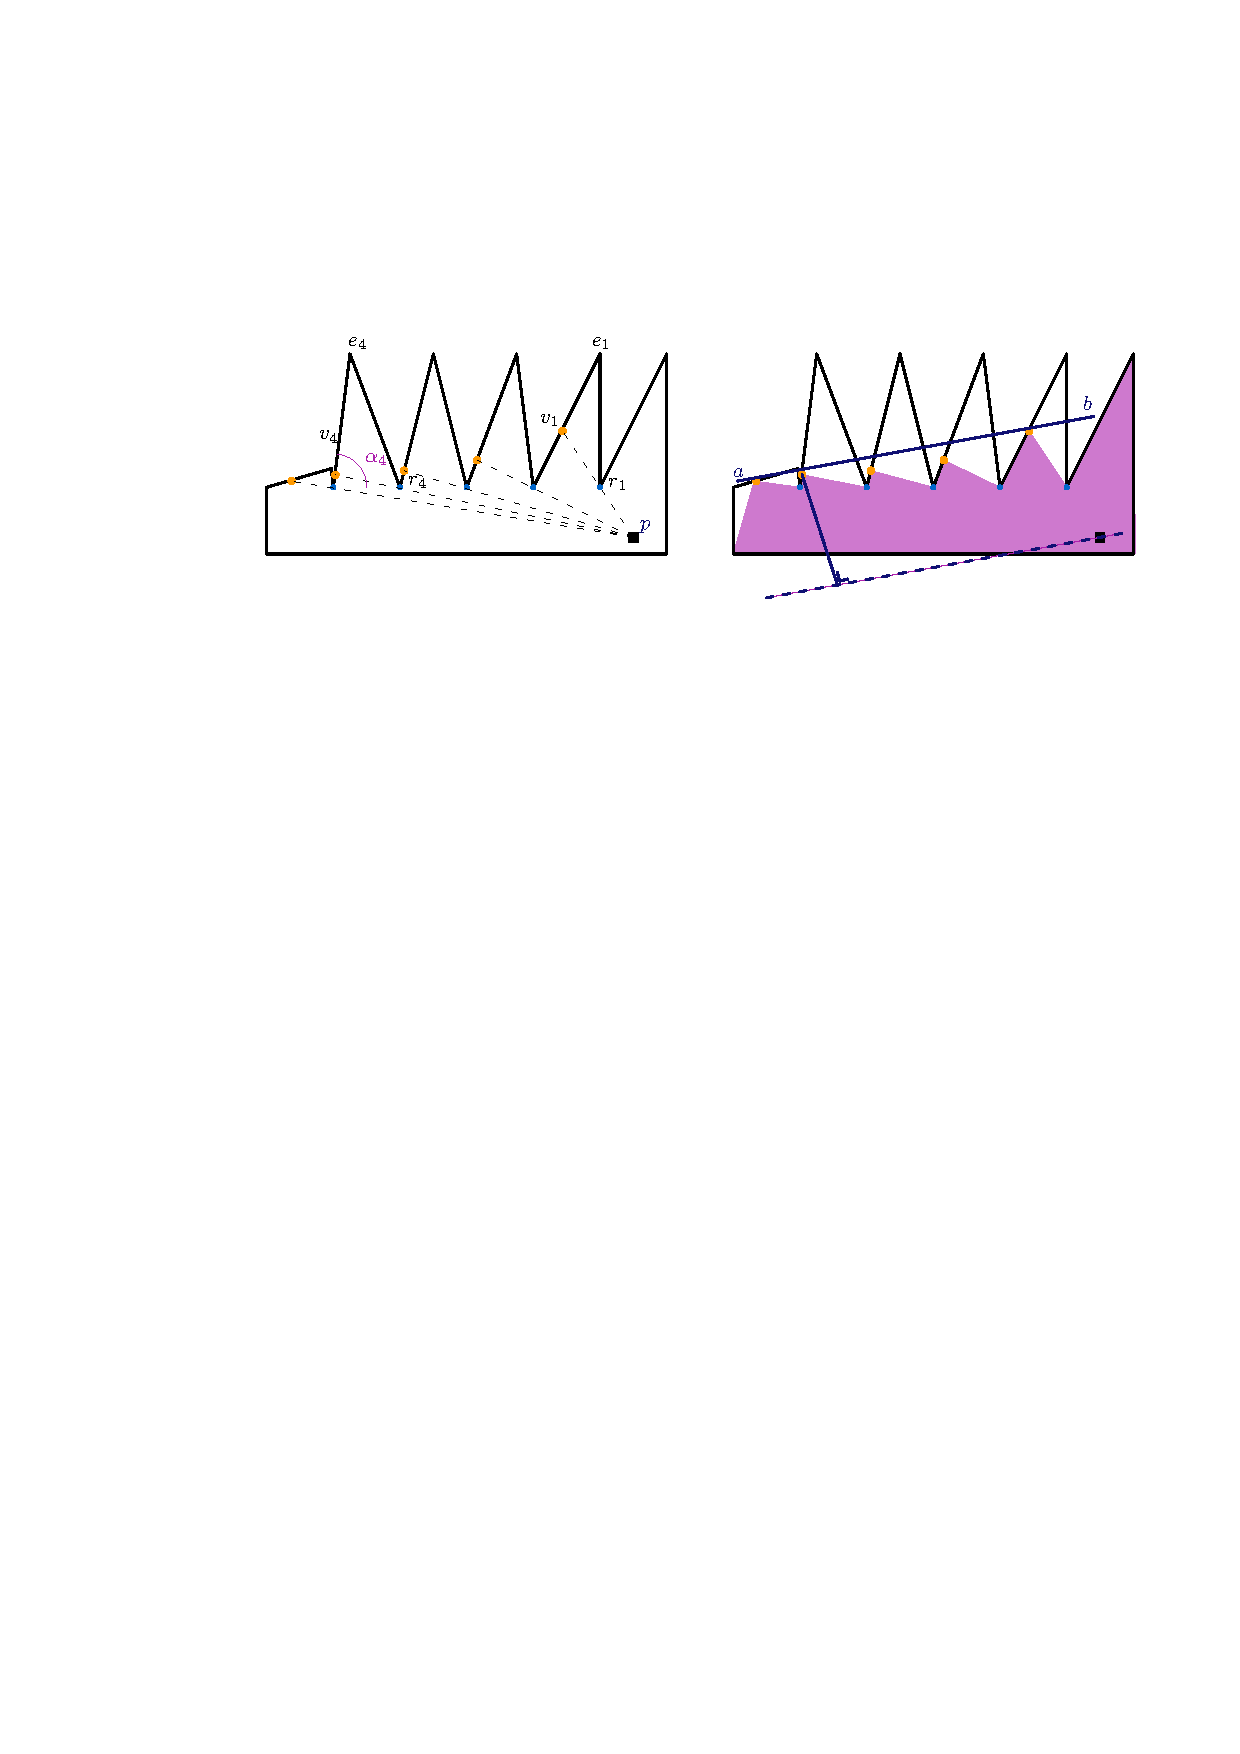
\includegraphics[]{starproblem}
  \caption{Here we see a star-shaped polygon $P$ and a donkey $p$ in $P$ as a big square. On the right we see the visibility polygon of $p$ in purple. In this case, the visibility polygon can be described as an alternating sequence between a reflex vertex $r_i$, and a following edge $e_i$ that is partially blocked by $r_i$ (ordered counterclockwise). The line from $p$ through $r_i$ onto $e_i$ lands in a vertex denoted by $v_i$, we call this vertex a \emph{final vertex}. The visibility polygon has as its vertices $r_i$ followed by $v_i$ in counterclockwise order. Suppose now that we have a query segment $a,b$ illustrated as in the right figure. If this segment intersects the visibility polygon, it cuts off the highest final vertex, where height is measured with respect to a line parallel to $ab$. The height of each $v_i$ is dependent $p$, $ab$ AND the slope that $e_i$ has. Moreover, note that if we marginally move $p$, each vertex $v_i$ starts moving upwards or downwards, depending on the slope of $e_i$. This makes it very hard to query which $v_i$ is maximal with respect to $ab$.}
    \label{fig:starproblem}
\end{figure}


\subsubsection{Polygonal Domain}
\begin{itemize}
    \item Is this harder than the simple polygon with walking through walls?
    \item Extend the data structure with more visibility constraints?
\end{itemize}


\subsubsection{Polygonal Domain with Walking Through Walls}
\begin{itemize}
    \item Is this any different to a polygonal domain without walking through walls?
\end{itemize}

\subsection{Two Alive Monkeys}

\subsubsection{In a Simple Polygon}
Some details and some pictures in Section 3.
\begin{itemize}
    \item For a given pair of query segments, compute the hourglass $\Xi$ between them using Guibas \& Hershberger and dualize it into a convex polygon $D(\Xi)$. This polygon must be represented implicitly as a data structure, which could cause a problem for any of the following steps if we're not careful.
    \item The line between $m_1(t)$ and $m_2(t)$ forms a point in the dual, for $t \in [0,1]$ the point traces out a segment of a hyperbola. If the hyperbola intersects $D(\Xi)$, then there's a moment of visibility.
    \item Since it is only a segment of a hyperbola we will have to ``crop'' $D(\Xi)$ by intersecting it with the half-plane through the endpoints of the hyperbola. We suppose this can be done without problems for some reason I don't remember.
    \item If the hyperbola intersects $D(\Xi)$ either it cuts off a vertex or it enters and leaves a single edge. The second case is simpler since there is only one edge the hyperbola can intersect. We can form a triangle which splits $D(\Xi)$ in half then determine whether the hyperbola is over or under the triangle and recurse to find the edge it could intersect, then check if it does.
    \item If the hyperbola cuts off a vertex then the problem becomes ``are there vertices of $D(\Xi)$ on both sides of the hyperbola?'' We can use semi-algebraic range searching (emptiness) with the vertices of $D(\Xi)$ as points and the hyperbola as a query to answer this in $O(\sqrt n)$ time. I think linearization is sufficient (since our query is degree $2$), and the fancy algebraic techniques of Agarwal \& Matoušek  are overkill. The details seem quite challenging, given we only have the points in a ``cropped'' data structure though.
    \item Maarten says: Hey, I thought it was not possible that the hyperbola curves with the polygon, or anti-curves with the polygon. One of the two?
\end{itemize}

\subsubsection{In a Polygonal Domain}
Some details and some pictures in Sections 4 and 5.
\begin{itemize}
    \item We can't form the hourglass between the query segments, since there could be linearly many distinct hourglasses, so any approach similar to the simple polygon method seems sunk.
    \item Instead form an hourglass (and thus a dualized convex polygon) for every pair of edges of the polygon or polygonal domain and intersect the query hyperbola with them. We can't do the intersection with the method used above, but we can probably use Sharir and Shaul's Stone Throwing problem to intersect the edges of the dual polygons \cite{SHARIR2005239}.
    \item However, not every hourglass we intersect is a good one as shown by some figures in Section 4. We need to intersect an hourglass and also have each monkey be inside the hourglass at the time of intersection. It seems we must introduce a time or distance based dimension to our problem.
    \item In Section 5 a solution is proposed which solves the problem by adding two additional dimensions to the dual space - for the min and max distances of an edge from some reference axis. This turns the convex polygons into ``hyper-cylinders'' of linear total complexity. Now the problem is again just a matter of an intersection, except in four dimensions. There seems some hope we can still use stone throwing.
    \item Seems possible that we can actually get by with only three dimensions, which might have big implications for the data structure we use. Since it's the order of edges which is most important we may only need to know the distance from a reference line. Frank, Martin and I discussed this at the workshop and I believed it then ... involves treating our dual polygons as belonging to layers, and at certain vertices the layers merge ...
    \item we can introduce a time element, but that seems to undo the very thing we were trying to achieve by considering the query hyperbola
\end{itemize}

Some questions:
\begin{itemize}
  \item What actually is harder about a polygon with holes vs just walking through walls? Anything?
  \item What about a polygonal domain where we can walk through walls, is that any different?
\end{itemize}

\section{Two alive monkeys that cannot walk through walls.}




Throughout this section we will refer as the $xy$-plane as the primal and the $ab$-plane as the dual. For any two points $\vec{p}, \vec{q}$ in the primal, denote  with $line(\vec{p}\vec{q})$ the line through and with $\overline{\vec{p}\vec{q}}$ the segment between $\vec{p}$ and $\vec{q}$.

There are two monkeys within a simple polygon $P$: The monkey $M_1$ that walks from $(a_1, a_2)$ to $(a_1 + a_3, a_2 + a_4)$ and the monkey $M_2$ that walks from  $(a_5, a_6)$ to $(a_5 + a_7, a_6 + a_8)$. Both monkeys walk with a (different) constant speed, such that they start  walking at time $0$ and stop walking at time $1$.  Thus we can parameterise the locations of monkeys with respect to a time $t \in [0,1]$ as: 

\begin{align*}
    \overline{M_1(t)} = \left( \begin{array}{c}
         x  \\
         y 
    \end{array}  \right) = \left( \begin{array}{c}
         a_1 + t a_3  \\
         a_2 + t a_4
    \end{array} \right)  \\
    \overline{M_2(t)} = \left( \begin{array}{c}
         x  \\
         y 
    \end{array}  \right) = \left( \begin{array}{c}
         a_5 + t a_7  \\
         a_6 + t a_8
    \end{array} \right)  \\
\end{align*}

At any time $t$, there is a line segment between the location of monkey 1: $M_1(t)$ and the location of monkey 2: $M_2(t)$. We denote this line segment by $\overline{h(t)}= \overline{M_1(t)M_2(t)}$ and the monkeys can see one another if and only if there is a time $t'$ such that $\overline{h(t')}$ is contained within $P$. This section has two subsections. Section~\ref{sec:nonghost} shows how one can compute if such a time $t'$ exists, using an intersection query in $\mathbb{R}^2$. Section~\ref{sec:linear} shows how to answer this intersection query in logarithmic time after preprocessing.


\subsection{From hourglass, to visibility glass, to intersection queries.}
\label{sec:nonghost}

Let $l_1$ and $l_2$ be two line segments that are contained in $P$ in the $xy$-plane. Guibas \etal define the \emph{hourglass} $H(l_1, l_2)$ of $l_1$ and $l_2$ as the area enclosed by $l_1, l_2$ and the shortest paths between the endpoints of $l_1$ and $l_2$. In \cite{GUIBAS1989126} Guibas \etal devise a linear-size data structure that for any pair $(l_1, l_2)$ can return the hourglass in logarithmic time, represented as a collection of trees where the leaves of these trees are the segments that form the hourglass.


We define the \emph{visibility glass} of $l_1$ and $l_2$ as follows: the visibility glass is the collection of lines that pass through $l_1$ and $l_2$, whose line segment between $l_1$ and $l_2$ is contained in $P$. $V(l_1, l_2) := \{ line(pq) \mid p \in l_1, q \in l_2,  \overline{pq} \subset P \}$. \\

\begin{lemma}
  For each pair of line segments $l_1, l_2 \in P$, there are two sub-segments $m_1, m_2$ of $l_1$ and $l_2$ respectively such that $H(m_1, m_2) = V(l_1, l_2)$. Moreover, given $l_1$ and $l_2$ we can identify $m_1$ and $m_2$ in logarithmic time and the visibility glass is a convex polygon of in the dual.
\end{lemma}

Each visibility glass $V(l_1, l_2)$ is a region in the $ab$-plane that represents a collection of lines that \emph{could} be a line-of-sight between the two monkeys. Thus, it is natural to ask what the line-of-sight of the monkeys looks like in this domain. Recall that in the previous section, we denoted by $h(t)$ the line that goes through $M_1(t)$ and $M_2(t)$. We can plot $h(t)$ in the $ab$-plane as a parameterised curve. For ease of notation we denote by $A_i = a_i - a_{i-4}$ (this is the coordinate of the second monkey, minus the coordinate of the first monkey):


  \begin{equation*}
   h(t) = \left( \begin{array}{c}
         a(t)  \\
         b(t) 
    \end{array}  \right) = 
    \left( \begin{array}{c}
         \frac{M_2(t).Y - M_1(t).Y}{M_2(t).X - M_1(t).X}  \\
         a(t)\cdot M_1(t).X - M_1(t).Y 
    \end{array}  \right) =
    \left( \begin{array}{c}
         \frac{ A_6 + A_8 t}
      { A_5  + A_7 t }  \\
         a(t)(a_1 - a_3 t) - a_2 - a_4 t 
    \end{array}  \right)
  \end{equation*}

Observe that the two monkeys can see one another, if and only if there is a time $t$ such that $h(t)$ intersects the visibility glass $V(M_1, M_2)$. $V(M_1, M_2)$ consists of at most $n$ edges in the $ab$-plane. Thus, we can rephrase our visibility query, into an intersection query between $n$ line segments in the plane and a curve $h(t)$.
We solve this new query, using the linearisation techniques from Agarwal \etal \cite{agarwal2013range}.

\section{Obtaining the Visibility Glass}

\subsection{Obtaining the Hourglass}

Suppose we have two line segments $\overline{p_1 p_2}$ and $\overline{q_1 q_2}$ in a simple polygon $P$. Let $\pi(a, b)$ be the shortest path between $a$ and $b$.

\begin{lemma}
    If $p_1$, $p_2$, $q_2$ and $q_1$ are in convex position, and w.l.o.g. appear in that order along their convex hull, the hourglass of $\overline{p_1 p_2}$ and $\overline{q_1 q_2}$ is the polygon whose perimeter is $\overline{p_1 p_2} \cup \pi(p_2, q_2) \cup \overline{q_1 q_2} \cup \pi(q_1, p_1)$.
    
    If, w.l.o.g. $p_1$, $p_2$ and $q_1$ are in convex position then the hourglass of $\overline{p_1 p_2}$ and $\overline{q_1 q_2}$ is the funnel with boundary $\overline{p_1 p_2} \cup \pi(p_1, q_1) \cup \pi(p_2, q_1)$.
\end{lemma}

\begin{proof}
This is ``obvious'' by convexity. If $q_2$ is on the convex hull then $\pi(p_2, p_1)$ must be ``above'' $\pi(p_2, q_2)$ and so cannot be extremal.
\end{proof}

Hence we build the Guibas and Hershberger data structure on $P$ then, given $p_1$, $p_2$, $q_1$ and $q_2$, check if they are in convex position in constant time, then in logarithmic time query Guibas and Hershberger to get a pointer to the trees for the top and bottom chains.

\subsection{Obtaining the Visibility Glass}
Given a hourglass we can turn it into a visbility glass in $O(\log n)$ using an algorithm from \cite{GuibasHS91}. It's a straightforward binary search.


\section{new linearization}




\section{Visibility as an intersection}


At time $t \in [0,1]$, the line segment $\overline{q(t)r(t)}$ is the line-of-sight between the two points. The points can see one another at time $t$ if and only if the segment $\overline{q(t)r(t)}$  is contained within the visibility glass $L(e_1, e_2)$. Therefore we can answer our query by checking if there is a time $t^*$ such that $\overline{q(t^*)r(t^*)}$ is contained in $L(e_1,e_2)$ (and therefore in $P$). We check this as follows:
it is known \cite{Chazelle1989} that the dual of the visibility glass is a
convex polygon with at most $n$ edges and we denote this polygon by
$\Lambda(e_1,e_2)$. For all $t \in [0,1]$, we denote the dual of the line
$q(t)r(t)$ by the point $(\alpha(t), \beta(t))$, this point traces out a curve
$\gamma(t)$ (Equation~\ref{eq:curve}). A point of the query curve $\gamma(t)$
is contained in $\Lambda(e_1,e_2)$ only if: either $\gamma(t)$ is contained in,
or intersects the boundary of $\Lambda(q,r)$.
If $\gamma(t)$ is contained in $\Lambda(e_1, e_2)$, the entities can always see one another and since this is easy to verify we assume that this is not the case. Thus we only need to check if there is a time $t^*$ such that $\gamma(t)$ intersects the border of $\Lambda(e_1, e_2)$. We answer this intersection query with the linarization techniques from Agarwal \etal \cite{agarwal2013range}. 


For ease of notation, we assume that the entity $q$ walks from $(a_1, a_2)$ to $(a_1 + a_3, a_2 + a_4)$ and that the entity $r$ walks from $(a_5, a_6)$ to $(a_5 + a_7, a_6 + a_8)$, 
both during the time interval $[0,1]$. Now we can parametrize the position of entity $q$ and $r$ as follows:

\begin{equation}
    \label{eq:line}
     q(t) = \left( \begin{array}{c}
         x_{q(t)}  \\
         y_{q(t)} 
    \end{array}  \right) = 
    \left( \begin{array}{c}
         a_1 + a_3 t \\
         a_2 + a_4 t
    \end{array}  \right)  \quad
      r(t) = \left( \begin{array}{c}
         x_{r(t)}  \\
         y_{r(t)} 
    \end{array}  \right) = 
    \left( \begin{array}{c}
         a_5 + a_7 t \\
         a_6 + a_8 t
    \end{array}  \right) 
\end{equation}


At all times, the line $\gamma(t)$ represents the line through $q(t)$ and $r(t)$. We say that at all times, $\gamma(t)$ has slope $\alpha(t)$ and offset $\beta(t)$. The parametrisation of $\gamma(t)$ then becomes:

\begin{equation}
\label{eq:curve}
   \gamma(t) = \left( \begin{array}{c}
         \alpha(t)  \\
         \beta(t) 
    \end{array}  \right) = 
    \left( \begin{array}{c}
         \frac{y_{r(t)} - y_{q(t)}}{x_{r(t)} - x_{q(t)}}  \\
         \alpha(t)\cdot x_{q(t)} - y_{q(t)}
    \end{array}  \right) =
    \left( \begin{array}{c}
         \frac{ a_6 - a_2 + (a_8 - a_4) t}
      { a_5 - a_1  + (a_7 - a_3) t }  \\
         \alpha(t)(a_1 - a_3 t) - a_2 - a_4 t 
    \end{array}  \right)
  \end{equation}
  
  First, we take the equation for $\beta(t)$ and isolate the time variable $t$.
  
\begin{align*}
    \beta(t) =  \alpha(t)(a_1 - a_3 t) - a_2 - a_4 t \Rightarrow \\
   (\alpha(t) a_3 + a_4) t = \alpha(t) a_1 - a_2  - \beta(t) \Rightarrow \\
   t = \frac{\alpha(t) a_1 - a_2  - \beta(t)}{\alpha(t) a_3 + a_4}
\end{align*}

Then, we take the equation for $\alpha(t)$, and substitute the value for $t$ into it.
\begin{align*}
    ( a_5 - a_1  + (a_7 - a_3) t) \alpha(t) =  a_6 - a_2 + (a_8 - a_4) t \Rightarrow \\
    (a_5 - a_1) \alpha(t) + (a_7 - a_3) t \alpha(t) = (a_6 - a_2) + (a_8 - a_4) t \Rightarrow \\
    \textnormal{subtituting the newfound value for t gives}: \\
    (a_3 a_5 - a_1 a_3 + a_1 a_7 - a_1 a_3)[\alpha(t)^2] + \\
    (a_4 a_5- a_2 a_7 - a_3 a_6  - a_1 a_8) [\alpha(t)] + \\
    (a_8 - a_4) [\beta(t)]    (- a_7 + a_3)[\alpha(t)\beta(t)] + \\
    (-a_4 a_6  + a_2 a_8)[1]
\end{align*}




























\section{Linearization}

Agarwal \etal state the following.
Suppose that you have a collection of $n$ objects parameterised by a vector $\vec{x}$ and that you have a query $Q$, which is parameterised by a vector $\vec{a}$ and we are interested in knowing if $Q$ intersects any of our $n$ objects.
Suppose that for each object $\vec{x}$ and each query $\vec{a}$ we can formulate the intersection by a predicate with the following form:

\begin{equation}
    \textit{There is an intersection } \iff F(\vec{x}, \vec{a}) = A_0(\vec{a}) + \sum_{i=1}^k A_i(\vec{a})f_i(\vec{x}) \le C
\end{equation}

Where $f_i$ and $A_i$ are polynomial functions only dependent on $
\vec{x}$ and $\vec{a}$ respectively. Then we can formulate this query as a halfspace range query in $\mathbb{R}^k$ where each object $\vec{x}$ gets sent to the $k$-dimensional point: $(f_1(\vec{x}), f_2(\vec{x}), \dots f_k(\vec{x}))$ and each query $A_i$ gets sent to the halfspace range:

\begin{equation}
    Halfspace(\vec{a}) = \left\{y \in \mathbb{R}^k \mid A_0(\vec{a})  + \sum_i^k A_i(\vec{a})y_i  \le C \right\}
\end{equation}

We will apply this technique, to the intersection question that we posed in the previous subsection. Where our objects are $n$ line segments, each parameterised by a vector $\vec{x} = (x_1, x_2, x_3, x_4)$ and where our query is the curve $h_{\vec{a}}(t)$ with $\vec{a} = (a_1, a_2, a_3, a_4, a_5, a_6, a_7, a_8)$ for $t \in [0,1]$.  For simplicity, we first show how we would do it, if our query was not a complicated curve $h(t)$ but instead also a line segment parameterised by $\vec{a} = (a_1, a_2, a_3, a_4)$:

\subsection{Intersecting segments with a segment}

Suppose that we have a collection $S$ of $n$ line segments in the $ab$-plane parametrized by $\vec{x} = (x_1, x_2, x_3, x_4)$ and a query line segment $Q(t)$ in the $ab$-plane that goes from $(a_1, a_2)$ to $(a_1 + a_3, a_2 + a_4)$ and we want to know if $Q(t)$ intersects a segment in $S$. Agarwal \etal devise a linearization of this intersection query that evaluates the cross product between a segment $s \in S$ and $Q(t)$ \cite{agarwal2013range}. This linearization gives them a halfspace range query in $\mathbb{R}^4$, but this approach obviously does not work if the query is not a line segment. We instead introduce a new approach that uses a rotation of the plane which will give us a linearization to $\mathbb{R}^3$ instead of $\mathbb{R}^4$.
Suppose we parametrize $Q$ by $t$:

\begin{equation}
        \overline{Q(t)} = \left( \begin{array}{c}
         a(t)  \\
         b(t) 
    \end{array}  \right) = \left( \begin{array}{c}
         a_1 +  a_3t  \\
         a_2 + a_4t 
    \end{array} \right)  \\
\end{equation}

In this section, we construct 4 consecutive predicates. Where a query segment $\vec{x}$ intersects the query $\vec{a}$ if and only if all four predicates hold:
\begin{itemize}
    \item $F_1(\vec{x}, \vec{y}) \ge 0$
    \item $F_2(\vec{x}, \vec{y}) \le 0$
    \item $F_3(\vec{x}, \vec{y}) \ge 0$
    \item $F_4(\vec{x}, \vec{y}) \le 0$
\end{itemize}

Each predicate gives a linearization to $\mathbb{R}^3$. Hence, we can solve this using 4 consecutive halfspace range queries in $\mathbb{R}^3$ using $n^3$ space and $\log n$ time.

\subsection{Expressing the intersection as predicates}

Suppose we are given $\vec{a}$ and a segment $s$ given by the parameter $\vec{x}$. We apply two transformations to the plane: First we translate the plane with the vector $-(x_1, x_2)$ such that $s$ starts at the origin. Then we rotate the plane with the rotation matrix $R(x_3, x_4)$ such that $s(t)$ points upwards. We denote the transformed query segment by $\overline{Q(t)}$ and $Q(t)$ intersects $s$ if and only if:

\begin{itemize}
    \item There exists a time $t^*$ such that the $a$-coordinate of $\overline{Q(t^*)} = 0$ (always) 
    \item $t^* \ge 0$ (predicate $F_1$)
    \item $t^* \le 1$ (predicate $F_2$)
    \item The $b$-coordinate of $\overline{Q(t^*)} \le \sqrt{x_3^2 + x_4^2}$ (which is the length of $s$) (predicate $F_3$)
    \item The $b$-coordinate of $\overline{Q(t^*)} \ge 0$ (predicate $F_4$)

\end{itemize}

This is what we will try to show in this subsection. The rotation matrix is given by:

\begin{equation}
    R(x_3,x_4) = \left( \begin{array}{cc}
         \cos \phi & -\sin \phi  \\
         \sin \phi & \cos \phi 
    \end{array} \right) \textit{ where } \phi = \arctan ( \frac{x_3}{x_4})
\end{equation}
If we apply our translation and rotation, we get a new segment $\overline{Q(t)}$ given by:

\begin{align*}
    &\overline{Q(t)} = R(x_3, x_4) \cdot (Q(t) - (x_1, x_2)) =  
    \left( \begin{array}{c}
         a  \\
         b 
    \end{array} \right) =  \left( \begin{array}{cc}
         \cos \phi & -\sin \phi  \\
         \sin \phi & \cos \phi 
    \end{array} \right)  \cdot \left( \begin{array}{c}
         a_1 - x_1 + t a_3  \\
         a_2 - x_2 + t a_4 
    \end{array} \right) \\
    %
    &\overline{Q(t)} = 
    \left(
    \begin{array}{c}
         a  \\
         b 
    \end{array}  \right) = 
    \left( \begin{array}{c}
         \cos \phi * (a_1 - x_1 + t a_3) - \sin \phi * ( a_2 - x_2 + t a_4 )  \\
         \sin \phi * (a_1 - x_1 + t a_3) + \cos \phi  * (a_2 - x_2 + t a_4) 
    \end{array} \right)
\end{align*}
The first thing that we do, is that we compute the time $t^*$ for which the $a$-coordinate of $\overline{Q(t)}$ is zero:

\begin{align*}
    a = 0 \Rightarrow \\
    - (a_3 \cos \phi  - a_4 \sin \phi)t^* = (a_1 - x_1)\cos \phi  - (a_2 - x_2)\sin \phi \Rightarrow \\
    %
    t^* = \frac{ (a_1 - x_1)\cos \phi  - (a_2 - x_2)\sin \phi}{ a_4 \sin \phi -a_3 \cos \phi}
\end{align*}

The first predicate verifies whether or not $t^*$ is greater or equal than $0$:

\begin{align*}
    &0 \le t \Rightarrow \\
    &0 \le F_1(\vec{x}, \vec{a}) = a_1\cos \phi - x_1\cos \phi  - a_2\sin \phi + x_2\sin \phi  \\
    %
    &0 = (0) + (1)[x_2 \sin \phi - x_1 \cos \phi] + (a_1) [ \cos \phi] + (a_2) [ - \sin \phi ] \\
    \textnormal{Hence we have a predicate } F_1 \textnormal{ Where }\\
    %
    &A_0(\vec{a}) = 0, \quad A_1(\vec{a}) = 1,\quad A_2(\vec{a}) = a_1,\quad A_3(\vec{a}) = a_2 \\
    %
    &f_1(\vec{x}) = x_2 \sin \phi - x_1 \cos \phi,\quad f_2(\vec{x}) = \cos \phi, \quad f_3(\vec{x}) = -\sin \phi
\end{align*}

The second predicate verifies whether or not $t^*$ is lesser or equal to $1$:

\begin{align*}
    &t \le 1 \Rightarrow \\
    &0  \ge a_1\cos \phi - x_1\cos \phi  - a_2\sin \phi + x_2\sin \phi - a_4 \sin \phi  + a_3 \cos \phi   \\
    %
    &0 \ge F_2(\vec{x}, \vec{a}) = (0) + (1)[ x_2\sin \phi - x_1\cos \phi] + (a_1 + a_3) [ \cos \phi] + (a_2 + a_4)[- \sin \phi] \\
    \textnormal{Hence we have a predicate } F_2 \textnormal{ Where } \\
    %
    &A_0(\vec{a}) = 0, \quad A_1(\vec{a}) = 1,\quad A_2(\vec{a}) = a_1 + a_3,\quad A_3(\vec{a}) = a_2 + a_4 \\
    %
    &f_1(\vec{x}) = x_2 \sin \phi - x_1 \cos \phi,\quad f_2(\vec{x}) = \cos \phi, \quad f_3(\vec{x}) = -\sin \phi
\end{align*}

The third predicate, verifies whether not the $y$ value of $\overline{Q(t^*)}$ lies below $\sqrt{x_3^2 + x_4^2}$:

\begin{align*}
    \overline{Q(t^*)}.Y = \sin \phi * (a_1 - x_1 + t^* a_3) + \cos \phi  * (a_2 - x_2 + t^* a_4)  \le \sqrt{x_3^2 + x_4^2} \Rightarrow \\
    %
     \sin \phi * (a_1 - x_1 + \left(\frac{ (a_1 - x_1)\cos \phi  - (a_2 - x_2)\sin \phi}{ a_4 \sin \phi -a_3 \cos \phi}\right) a_3) + \\
     %
     \cos \phi  * (a_2 - x_2 + \left(\frac{ (a_1 - x_1)\cos \phi  - (a_2 - x_2)\sin \phi}{ a_4 \sin \phi -a_3 \cos \phi}\right) a_4) \le \sqrt{x_3^2 + x_4^2} 
\end{align*}

We multiply both sides by $(a_4 \sin \phi -a_3 \cos \phi)$ and obtain:


\begin{align*}
    a_1 \sin \phi (a_4 \sin \phi -a_3 \cos \phi) - x_1 \sin \phi (a_4 \sin \phi -a_3 \cos \phi)  \\
    %
    + ((a_1 - x_1)\cos \phi  - (a_2 - x_2)\sin \phi) a_3 \sin \phi \\
    %
    + a_2 \cos \phi (a_4 \sin \phi -a_3 \cos \phi) - x_2 \cos \phi (a_4 \sin \phi -a_3 \cos \phi) \\
    %
    + ((a_1 - x_1)\cos \phi  - (a_2 - x_2)\sin \phi) a_4 \cos \phi \\
    %
    \le  \sqrt{x_1, x_2}(a_4 \sin \phi -a_3 \cos \phi)\\
    %
\end{align*}
We can remove the brackets from this equation to detect redundancies (shown with underline). We also denote by $()$ the $A$-polynomials and by $[]$ the $f$-polynomials:

\begin{align*}
   F_3(\vec{a}, \vec{x}) = (a_1 a_4)[\sin^2 \phi] + \underline{(a_1 a_3)[- \sin \phi \cos \phi]} + \\
    %
    (a_4) [- x_1 \sin^2 \phi] + \underline{(a_3)[x_1 \sin \phi \cos \phi]} + \\
    %
    \underline{(a_1 a_3)[\sin \phi \cos \phi]} + \underline{(a_3)[-x_1 \sin \phi \cos \phi]} + \\
    %
    (a_2 a_3)[-\sin^2 \phi] + (a_3)[x_2 \sin^2 \phi] + \\
    %
    \underline{(a_2 a_4)[\sin \phi \cos \phi]} + (a_2 a_3)[-\cos^2 \phi] + \\
    %
    \underline{(a_4)[-x_2 \sin \phi \cos \phi]} + (a_3)[x_2 \cos^2 \phi] + \\
    %
    (a_1 a_4)[\cos^2 \phi] + (a_4)[-x_1 \cos^2 \phi] + \\
    %
    \underline{(a_2 a_4)[-\sin \phi \cos \phi]} + \underline{(a_4)[x_2 \sin \phi \cos \phi]} + \\
    %
    (a_4)[\sqrt{x_1 + x_2}\sin \phi] + (a_3)[-\sqrt{x_1 + x_2}\cos \phi] \le 0
\end{align*}

Having removed these redundant terms, we note that we see several $A$-polynomials which are attached to the same $f$-polynomial and we join them into new $A$-polynomials:

\begin{align*}
    F_3(\vec{a}, \vec{x}) = (a_1 a_4 - a_2 a_3)[\sin^2 \phi] +     (a_4) [- x_1 \sin^2 \phi] +    (a_3)[x_2 \sin^2 \phi] + \\
   (a_1 a_4 - a_2a_3)[\cos^2 \phi] + (a_3)[x_2\cos^2 \phi] + (a_4)[-x_1 \cos^2 \phi] + \\
    %
    (a_4)[-\sqrt{x_3 + x_4}\sin \phi] + (a_3)[\sqrt{x_3 + x_4}\cos \phi] \le 0
\end{align*}

We note that there are several $f$-polynomials which are attached to the $A$-polynomial $a_3$ or $a_4$ and we also join these: 

\begin{align*}
    F_3(\vec{a}, \vec{x}) = (a_1 a_4 - a_2 a_3)[\sin^2 \phi + \cos^2 \phi]  \\
    + (a_4) [- x_1 \sin^2 \phi - x_1 \cos^2 \phi -\sqrt{x_3 + x_4}\sin \phi ]  \\  + (a_3)[x_2 \sin^2 \phi + x_2\cos^2 \phi+ \sqrt{x_3 + x_4}\cos \phi]  \le 0
\end{align*}

Lastly we conclude (with noting that $\sin^2 \phi + \cos^2 \phi = 1$):

\begin{align*}
    &F_3(\vec{a}, \vec{x}) = (a_1 a_4 - a_2 a_3)[\sin^2 \phi] + (a_1 a_4 - a_2a_3)[\cos^2 \phi]  \\
    &+ (a_4) [- x_1 -\sqrt{x_1 + x_2}\sin \phi ]  \\  
    &+ (a_3)x_2 + \sqrt{x_1 + x_2}\cos \phi]  \le 0 \\
      &\textnormal{Hence we have a predicate } F_3 \textnormal{ Where } \\
    %
    &A_0(\vec{a}) = 0, \quad A_1(\vec{a}) = a_1 a_4 - a_2 a_3,\quad A_2(\vec{a}) = a_2 a_3 - a_1 a_4,\quad A_3(\vec{a}) = a_3, \quad  A_4(\vec{a})= a_4\\
    %
    &f_1(\vec{x}) = \sin^2 \phi,\quad f_2(\vec{x}) = \cos^2 \phi, \quad f_3(\vec{x}) = x_2 + \sqrt{x_3 + x_4}\cos \phi, \quad f_4(\vec{x}) = -x_1-\sqrt{x_3 + x_4}
\end{align*}

Which means that we can solve this intersection query with a linearisation to $\mathbb{R}^4$.
\newpage 

intentionally left blank

\newpage
\subsection{Linearization of a hyperbolic curve}

We now apply the same transformation to the hyperbola $H(t)$. For conveciency, we define new $a$-variables:
$A_i = a_i - a_{i-4}$.
The formula for $H(t)$ now becomes:

\begin{equation}
  H(t) = \left( \begin{array}{c}
         a  \\
         b 
    \end{array}  \right) =  
        \left( \begin{array}{c}
         \frac{ A_6 + A_8 t}
      { A_5  + A_7 t } \\
         a(t)(a_1 +  a_3 t) - a_2 -  a_4 t 
    \end{array}  \right)
\end{equation}

Removing brackets and applying the transformation gives:

  \begin{equation*}
   H_T(t) = \left( \begin{array}{c}
         a  \\
         b 
    \end{array}  \right) = 
    \left( \begin{array}{c}
         \frac{ A_6 + A_8 t}
      { A_5  + A_7 t } - x_1 \\
         \frac{ A_6 a_1 + A_8 a_1 t + A_6 a_3 t + A_8 a_3 t^2 }{A_5 + A_7t} - a_2 - a_4 t - x_2
    \end{array}  \right)
  \end{equation*}
  
We then apply the rotation matrix and obtain $\overline{H(t)}$:

\begin{equation*}
   \overline{H(t)} = \left( \begin{array}{c}
         a  \\
         b 
    \end{array}  \right) = 
    \left( \begin{array}{c}
        \cos \phi \left(\frac{ A_6 + A_8 t}
      { A_5  + A_7 t } - x_1 \right) - \sin \phi \left(\frac{ A_6 a_1 + A_8 a_1 t + A_6 a_3 t + A_8 a_3 t^2 }{A_5 + A_7t} - a_2 - a_4 t - x_2 \right) \\
      %
         \sin \phi \left(\frac{ A_6 + A_8 t}
      { A_5  + A_7 t } - x_1 \right)  + \cos \phi \left( \frac{ A_6 a_1 + A_8 a_1 t + A_6 a_3 t + A_8 a_3 t^2 }{A_5 + A_7t} - a_2 - a_4 t - x_2 \right)
    \end{array}  \right)
\end{equation*}

\subsection{Verifying that $0 \le t^* \le 1$}

The first thing that we do, is verify the time $t^*$ for which $a=0$ and check whether that value lies below 1. We do this by multiplying each side of the inequality with $(A_5 + A_7 t)$.

\begin{align*}
    &\cos \phi \left(\frac{ A_6 + A_8 t}
      { A_5  + A_7 t } - x_1 \right) - \sin \phi \left(\frac{ A_6 a_1 + A_8 a_1 t + A_6 a_3 t + A_8 a_3 t^2 }{A_5 + A_7t} - a_2 - a_4 t - x_2 \right) = 0 \Rightarrow \\
      %
     &\cos \phi (A_6 - A_5x_1 + A_8t - A_7 x_1 t ) - \\
     %
      &\sin \phi (A_6 a_1 - A_5a_2 - A_5x_2 + A_8 a_1  t +   A_6 a_3 t  - A_7a_2 t - A_5a_4 t- A_7x_2 t+ A_8 a_3 t^2  -A_7a_4 t^2 ) = 0 \Rightarrow \\
      %
      %ABC-formulation incoming
      &[t^2] (a_3A_8 -a_4A_7 )\sin \phi + \\
      &[t] ( (A_8 -  A_7 x_1) \cos \phi - 
      (a_1A_8  +   a_3A_6   - a_2A_7 - a_4A_5- x_2A_7) \sin \phi) +\\
      &[1] (  (A_6 -  A_5 x_1) \cos \phi -
      (a_1A_6  - a_2A_5 - A_5x_2) \sin \phi ) = 0
\end{align*}

I see no other way to solve this, other than slamming it into the ABC formula.




If we want to equate $t$ thing lesser or equal to 1, we can write the following:

\begin{align*}
     1 \ge abc-formula \Rightarrow \\
    2c \ge -b + \sqrt{b^2 - 4 ac} \Rightarrow \\
    4c^2 + 4bc + b^2 \ge b^2 - 4 ac \Rightarrow \\
    (c^2 - bc + ac) \ge 0 
\end{align*}

\paragraph*{Working out $c^2$:}

\begin{align*}
    c^2 = (  (  (A_6 -  A_5 x_1) [\cos \phi] -
      (a_1A_6  - a_2A_5 - A_5x_2) [\sin \phi] )^2 = \\
      %
          ((A_5^2) x_1^2 - (2 A_5 A_6) x_1  + A_6^2)[\cos^2 \phi] +\\
          %
    ( (2 a_2 A_5^2 - 2 a_1 A_6 A_5) x_2 + (A_5^2) x_2^2 
    +  (a_2^2 A_5^2 - 2 a_1 a_2 A_6 A_5 + a_1^2 A_6^2)    ) [\sin^2 \phi] + \\
    %
    ((a_1 A_6 A_5 -a_2 A_5^2 ) x_1 - (A_5^2) x_1 x_2 + (A_6 A_5) x_2 + (a_2 A_6 A_5 - a_1 A_6^2) ) [\cos \phi \sin \phi]
\end{align*}


\paragraph*{Working out the $ac$:}

\begin{align*}
    ac = (A_8 a_3-A_7a_4 )[\sin \phi] \cdot
    (  (A_6 -  A_5 x_1) [\cos \phi] - (a_1A_6  - a_2A_5 - A_5x_2) [\sin \phi] )  \\
    %
    ( (a_3 A_5 A_8-a_4 A_5 A_7) x_2 + ( - a_2 a_4 A_5 A_7 + a_1 a_4 A_6 A_7 + a_2 a_3 A_5 A_8 - a_1 a_3 A_6 A_8) ) [\sin^2 \phi] + \\
    %
    ((a_4 A_5 A_7 - a_3 A_5 A_8)x_1  + (a_3 A_6 A_8- a_4 A_6 A_7) ) [\sin \phi \cos \phi]
\end{align*}

\paragraph{Working out the $bc$:}

\begin{align*}
     bc = ( (A_8 -  A_7 x_1) [\cos \phi] - 
      (a_1A_8  +   a_3A_6   - a_2A_7 - a_4A_5- x_2A_7) [\sin \phi]) \cdot \\
      (  (A_6 -  A_5 x_1) \cos \phi -
      (a_1A_6  - a_2A_5 - A_5x_2) \sin \phi ) = \\
      (A_5 A_7 x_1^2 + (- A_6 A_7 - A_5 A_8) x_1 + A_6 A_8) [\cos^2 \phi] + \\
      ( A_5 A_7 x_2^2 + (-a_1 A_6 A_7 - a_1 A_5 A_8 + a_4 A_5^2 - a_3 A_5 A_6 + 2 a_2 A_5 A_7)x_2 + \\
      (a_1^2 A_6 A_8 + a_3 a_1 A_6^2 - a_4 a_1 A_5 A_6 - a_2 a_1 A_6 A_7 - a_2 a_1 A_5 A_8 + a_2 a_4 A_5^2 - a_2 a_3 A_5 A_6 + a_2^2 A_5 A_7)) [\sin^2 \phi] + \\
      (-a_4 A_5^2 + a_3 A_6 A_5 - 2 a_2 A_7 A_5 + a_1 A_8 A_5 + a_1 A_6 A_7)x_1 + \\
      + (A_8 A_5+A_6 A_7) x_2 + (-2 A_7 A_5) x_1 x_2 + \\
      (a_4 A_6 A_5 + a_2 A_8 A_5 - a_3 A_6^2 + a_2 A_6 A_7 - 2 a_1 A_6 A_8) [\sin \phi \cos \phi]
\end{align*}


Now we work out the terms, per $\sin$-term:



\paragraph*{$\cos^2 \phi$:}

\begin{align*}
    &[[\cos^2 \phi]] \cdot  \\
       &[ x_2^2] (0) \\
    \quad \\
    &[x_1^2] ((A_5^2) + A_5 A_7) \\
    \quad \\
    &[x_2] (0) \\
    \quad \\
    &[x_1] ((-2 A_5 A_6) - (A_5 A_8 + A_6 A_7) ) \\
    \quad \\
    &[x_1 x_2] (0) \\
    \quad \\
   &[1] ( A_6^2 + A_6 A_8 )
\end{align*}

Giving 3 terms.


\paragraph*{$\sin^2 \phi$:}

\begin{align*}
    &[[\sin^2 \phi]] \cdot \\
    &([x_2^2] (A_5 A_7) \\
    \quad \\
    &[x_1^2] (0) \\
    \quad \\
    &[x_2] ( (a_3 A_5 A_8-a_4 A_5 A_7) + (-a_1 A_6 A_7 - a_1 A_5 A_8 + a_4 A_5^2 - a_3 A_5 A_6 + 2 a_2 A_5 A_7)) \\
    \quad \\
    &[x_1] (0) \\
    \quad \\
    &[x_1 x_2] (0) \\
    \quad \\
    &[1] ((a_1^2 A_6 A_8 + a_3 a_1 A_6^2 - a_4 a_1 A_5 A_6 - a_2 a_1 A_6 A_7 - a_2 a_1 A_5 A_8 + a_2 a_4 A_5^2 - a_2 a_3 A_5 A_6 + a_2^2 A_5 A_7) + \\
    &( - a_2 a_4 A_5 A_7 + a_1 a_4 A_6 A_7 + a_2 a_3 A_5 A_8 - a_1 a_3 A_6 A_8) ) )
\end{align*}

Giving 3 terms.


\paragraph*{$\sin \phi \cos \phi$:}


\begin{align*}
    &[[\sin \phi \cos \phi]] \cdot  \\
        &[x_2^2](0) \\
    \quad \\
    &[x_1^2] (0) \\
    \quad \\
    &[x_2] ((A_8 A_5+A_6 A_7) + (A_6 A_5)) \\
    \quad \\
    &[x_1] ((-a_4 A_5^2 + a_3 A_6 A_5 - 2 a_2 A_7 A_5 + a_1 A_8 A_5 + a_1 A_6 A_7) + \\
    &(a_4 A_5 A_7 - a_3 A_5 A_8) +(a_1 A_6 A_5 -a_2 A_5^2 )) \\
    \quad \\
    &[x_1 x_2] (-2 A_7 A_5 - A_5^2) \\
    \quad \\
    &[1] ((a_4 A_6 A_5 + a_2 A_8 A_5 - a_3 A_6^2 + a_2 A_6 A_7 - 2 a_1 A_6 A_8) + \\
    &(a_3 A_6 A_8- a_4 A_6 A_7)+ (a_2 A_6 A_5 - a_1 A_6^2))
\end{align*}

Giving 4 terms.



So we have a predicate for the first two checks:

$F(\vec{x}, \vec{a}) = \sum terms \ge 0$ with a total of 10 terms. Giving a halfspace range query of 10 dimensions. 
Note that the check if $t^* \ge 0$ has fewer terms than the check $t^* \le 1$.


\newpage

Page intentionally left blank.
\newpage


\subsection{Determining the intersection.}

We know that $t^* = \frac{-b \pm \sqrt{b^2 - 4ac}}{2c}$ and with the previous predicate, we can determine if $t^*$ lies within the relevant interval. The next step is to check if at time $t^*$, the $b$-value of the hyperbola is between $0$ and $C = \sqrt{x_3^2 + x_4^2}$.


\begin{align*}
     b \le C \Rightarrow \\
             \sin \phi \left(\frac{ A_6 + A_8 t}
      { A_5  + A_7 t } - x_1 \right)  + \cos \phi \left( \frac{ a_1A_6 + a_1A_8 t +  a_3A_6 t +  a_3A_8 (t)^2 }{A_5 + A_7t} - a_2 - a_4 t - x_2 \right)  \le C \Rightarrow \\
      \sin \phi (A_6 + A_8 t  - A_5x_1  + A_7 x_1 t ) + 
      \cos \phi ( a_1A_6 + a_1 A_8 t +  a_3A_6 t +  a_3A_8 (t)^2  \\
      - a_2 A_7t - a_4A_7 (t)^2 - A_7 x_2 t - a_2A_5 - a_4A_5 t - A_5x_2) - C(A_5) - CA_7t \le 0 \Rightarrow \\
      \quad \\
      \textnormal{Grouping variables on t} \\
      %t^2
      [t^2] \cos \phi( a_3A_8- a_4A_7 ) + \\
      [t]  ( \sin \phi (A_8 + A_7 x_1) +
      \cos \phi (a_1 A_8 + a_3A_6 - a_2 A_7 - A_7 x_2- a_4A_5)- C(A_5)) + \\
      [1] ( \sin \phi (A_6  - A_5x_1) + 
      \cos \phi ( a_1A_6- a_2A_5  - A_5x_2) - CA_7 )
    \textnormal{Substituting for the correct t value and multiplying with 4c2}:\\
          [b^2 - b\sqrt{D} + b^2 - 4ac] \cos \phi( a_3A_8- a_4A_7 ) + \\
      [-2bc + 2c\sqrt{D}]  ( \sin \phi (A_8 + A_7 x_1) +
      \cos \phi (a_1 A_8 + a_3A_6 - a_2 A_7 - A_7 x_2- a_4A_5)- C(A_5)) + \\
      [4c^2] ( \sin \phi (A_6  - A_5x_1) + 
      \cos \phi ( a_1A_6- a_2A_5  - A_5x_2) - CA_7 )
\end{align*}

Now it is clear that if you take $\sqrt{D}$ to one side and square, you get at least $b^4$ times a polynomial dependent on $x$ and $\vec{a}$. 

\newpage

Page intentionally left blank.
\newpage



\section{Shearing two alive monkeys.}




Throughout this section we will refer as the $xy$-plane as the primal and the $ab$-plane as the dual. For any two points $\vec{p}, \vec{q}$ in the primal, denote  with $line(\vec{p}\vec{q})$ the line through and with $\overline{\vec{p}\vec{q}}$ the segment between $\vec{p}$ and $\vec{q}$.

There are two monkeys within a simple polygon $P$: The monkey $q$ that walks from $(a_1, a_2)$ to $(a_1 + a_3, a_2 + a_4)$ and the monkey $r$ that walks from  $(a_5, a_6)$ to $(a_5 + a_7, a_6 + a_8)$. Both monkeys walk with a (different) constant speed, such that they start  walking at time $0$ and stop walking at time $1$.  Thus we can parameterise the locations of monkeys with respect to a time $t \in [0,1]$ as: 

\begin{align*}
    \overline{q(t)} = \left( \begin{array}{c}
         x  \\
         y 
    \end{array}  \right) = \left( \begin{array}{c}
         a_1 + t a_3  \\
         a_2 + t a_4
    \end{array} \right)  \\
    \overline{r(t)} = \left( \begin{array}{c}
         x  \\
         y 
    \end{array}  \right) = \left( \begin{array}{c}
         a_5 + t a_7  \\
         a_6 + t a_8
    \end{array} \right)  \\
\end{align*}

At any time $t$, there is a line segment between the two monkeys $\overline{h(t)}= \overline{q(t)r(t)}$ and the monkeys can see one another if and only if there is a time $t'$ such that $\overline{h(t')}$ is contained within $P$. This section has two subsections. Section~\ref{sec:nonghost} shows how one can compute if such a time $t'$ exists, using an intersection query in $\mathbb{R}^2$. Section~\ref{sec:linear} shows how to answer this intersection query in logarithmic time after preprocessing.


\subsection{From hourglass, to visibility glass, to intersection queries.}
\label{sec:nonghost}

Let $l_1$ and $l_2$ be two line segments that are contained in $P$ in the $xy$-plane. Guibas \etal define the \emph{hourglass} $H(l_1, l_2)$ of $l_1$ and $l_2$ as the area enclosed by $l_1, l_2$ and the shortest paths between the endpoints of $l_1$ and $l_2$. In \cite{GUIBAS1989126} Guibas \etal devise a linear-size data structure that for any pair $(l_1, l_2)$ can return the hourglass in logarithmic time, represented as a collection of trees where the leaves of these trees are the segments that form the hourglass.


We define the \emph{visibility glass} of $l_1$ and $l_2$ as follows: the visibility glass is the collection of lines that pass through $l_1$ and $l_2$, whose line segment between $l_1$ and $l_2$ is contained in $P$. $V(l_1, l_2) := \{ line(pq) \mid p \in l_1, q \in l_2,  \overline{pq} \subset P \}$. \\

\begin{lemma}
  For each pair of line segments $l_1, l_2 \in P$, there are two sub-segments $m_1, m_2$ of $l_1$ and $l_2$ respectively such that $H(m_1, m_2) = V(l_1, l_2)$. Moreover, given $l_1$ and $l_2$ we can identify $m_1$ and $m_2$ in logarithmic time and the visibility glass is a convex polygon of in the dual.
\end{lemma}

Each visibility glass $V(l_1, l_2)$ is a region in the $ab$-plane that represents a collection of lines that \emph{could} be a line-of-sight between the two monkeys. Thus, it is natural to ask what the line-of-sight of the monkeys looks like in this domain. Recall that in the previous section, we denoted by $h(t)$ the line that goes through $q(t)$ and $r(t)$. We can plot $h(t)$ in the $ab$-plane as a parameterised curve. For ease of notation we denote by $A_i = a_i - a_{i-4}$ (this is the coordinate of the second monkey, minus the coordinate of the first monkey):


  \begin{equation*}
   h(t) = \left( \begin{array}{c}
         a(t)  \\
         b(t) 
    \end{array}  \right) = 
    \left( \begin{array}{c}
         \frac{y_{r(t)} - y_{q(t)}}{x_{r(t)} - x_{q(t)}}  \\
         a(t)\cdot x_{q(t)} - y_{q(t)}
    \end{array}  \right) =
    \left( \begin{array}{c}
         \frac{ A_6 + A_8 t}
      { A_5  + A_7 t }  \\
         a(t)(a_1 - a_3 t) - a_2 - a_4 t 
    \end{array}  \right)
  \end{equation*}

Observe that the two monkeys can see one another, if and only if there is a time $t$ such that $h(t)$ intersects the visibility glass $V(q, r)$. $V(q, r)$ consists of at most $n$ edges in the $ab$-plane. Thus, we can rephrase our visibility query, into an intersection query between $n$ line segments in the plane and a curve $h(t)$.
We solve this new query, using the linearisation techniques from Agarwal \etal \cite{agarwal2013range}.

\section{Obtaining the Visibility Glass}

\subsection{Obtaining the Hourglass}

Suppose we have two line segments $\overline{p_1 p_2}$ and $\overline{q_1 q_2}$ in a simple polygon $P$. Let $\pi(a, b)$ be the shortest path between $a$ and $b$.

\begin{lemma}
    If $p_1$, $p_2$, $q_2$ and $q_1$ are in convex position, and w.l.o.g. appear in that order along their convex hull, the hourglass of $\overline{p_1 p_2}$ and $\overline{q_1 q_2}$ is the polygon whose perimeter is $\overline{p_1 p_2} \cup \pi(p_2, q_2) \cup \overline{q_1 q_2} \cup \pi(q_1, p_1)$.
    
    If, w.l.o.g. $p_1$, $p_2$ and $q_1$ are in convex position then the hourglass of $\overline{p_1 p_2}$ and $\overline{q_1 q_2}$ is the funnel with boundary $\overline{p_1 p_2} \cup \pi(p_1, q_1) \cup \pi(p_2, q_1)$.
\end{lemma}

\begin{proof}
This is ``obvious'' by convexity. If $q_2$ is on the convex hull then $\pi(p_2, p_1)$ must be ``above'' $\pi(p_2, q_2)$ and so cannot be extremal.
\end{proof}

Hence we build the Guibas and Hershberger data structure on $P$ then, given $p_1$, $p_2$, $q_1$ and $q_2$, check if they are in convex position in constant time, then in logarithmic time query Guibas and Hershberger to get a pointer to the trees for the top and bottom chains.

\subsection{Obtaining the Visibility Glass}
Given a hourglass we can turn it into a visbility glass in $O(\log n)$ using an algorithm from \cite{GuibasHS91}. It's a straightforward binary search.

\section{Linearization}

Agarwal \etal state the following.
Suppose that you have a collection of $n$ objects parameterised by a vector $\vec{x}$ and that you have a query $Q$, which is parameterised by a vector $\vec{a}$ and we are interested in knowing if $Q$ intersects any of our $n$ objects.
Suppose that for each object $\vec{x}$ and each query $\vec{a}$ we can formulate the intersection by a predicate with the following form:

\begin{equation}
    \textit{There is an intersection } \iff F(\vec{x}, \vec{a}) = A_0(\vec{a}) + \sum_{i=1}^k A_i(\vec{a})f_i(\vec{x}) \le C
\end{equation}

Where $f_i$ and $A_i$ are polynomial functions only dependent on $
\vec{x}$ and $\vec{a}$ respectively. Then we can formulate this query as a halfspace range query in $\mathbb{R}^k$ where each object $\vec{x}$ gets sent to the $k$-dimensional point: $(f_1(\vec{x}), f_2(\vec{x}), \dots f_k(\vec{x}))$ and each query $A_i$ gets sent to the halfspace range:

\begin{equation}
    Halfspace(\vec{a}) = \left\{y \in \mathbb{R}^k \mid A_0(\vec{a})  + \sum_i^k A_i(\vec{a})y_i  \le C \right\}
\end{equation}

We will apply this technique, to the intersection question that we posed in the previous subsection. Where our objects are $n$ line segments, each parameterised by a vector $\vec{x} = (x_1, x_2, x_3, x_4)$ and where our query is the curve $h_{\vec{a}}(t)$ with $\vec{a} = (a_1, a_2, a_3, a_4, a_5, a_6, a_7, a_8)$ for $t \in [0,1]$.  For simplicity, we first show how we would do it, if our query was not a complicated curve $h(t)$ but instead also a line segment parameterised by $\vec{a} = (a_1, a_2, a_3, a_4)$:

\subsection{Intersecting segments with a segment}

Suppose that we have a collection $S$ of $n$ line segments in the $ab$-plane parametrized by $\vec{x} = (x_1, x_2, x_3, x_4)$ and a query line segment $Q(t)$ in the $ab$-plane that goes from $(a_1, a_2)$ to $(a_1 + a_3, a_2 + a_4)$ and we want to know if $Q(t)$ intersects a segment in $S$. Agarwal \etal devise a linearization of this intersection query that evaluates the cross product between a segment $s \in S$ and $Q(t)$ \cite{agarwal2013range}. This linearization gives them a halfspace range query in $\mathbb{R}^4$, but this approach obviously does not work if the query is not a line segment. We instead introduce a new approach that uses a shearing of the plane which will give us a linearization to $\mathbb{R}^3$ instead of $\mathbb{R}^4$.
Suppose we parametrize $Q$ by $t$:

\begin{equation}
        \overline{Q(t)} = \left( \begin{array}{c}
         a(t)  \\
         b(t) 
    \end{array}  \right) = \left( \begin{array}{c}
         a_1 +  a_3t  \\
         a_2 + a_4t 
    \end{array} \right)  \\
\end{equation}

In this section, we construct 4 consecutive predicates. Where a query segment $\vec{x}$ intersects the query $\vec{a}$ if and only if all four predicates hold:
\begin{itemize}
    \item $F_1(\vec{x}, \vec{y}) \ge 0$
    \item $F_2(\vec{x}, \vec{y}) \le 0$
    \item $F_3(\vec{x}, \vec{y}) \ge 0$
    \item $F_4(\vec{x}, \vec{y}) \le 0$
\end{itemize}

Each predicate gives a linearization to $\mathbb{R}^3$. Hence, we can solve this using 4 consecutive halfspace range queries in $\mathbb{R}^3$ using $n^3$ space and $\log n$ time.

\subsection{Expressing the intersection as predicates}

Suppose we are given $\vec{a}$ and a segment $s$ given by the parameter $\vec{x}$. We apply two transformations to the plane: First we translate the plane with the vector $-(x_1, x_2)$ such that $s$ starts at the origin. Then we shear the plane with the following map: $(x,y) \rightarrow (x - \frac{x_3}{x_4}y, y)$ such that $s(t)$ points upwards. We denote the transformed query segment by $\overline{Q(t)}$ and $Q(t)$ intersects $s$ if and only if:

\begin{itemize}
    \item There exists a time $t^*$ such that the $a$-coordinate of $\overline{Q(t^*)} = 0$ (always) 
    \item $t^* \ge 0$ (predicate $F_1$)
    \item $t^* \le 1$ (predicate $F_2$)
    \item The $b$-coordinate of $\overline{Q(t^*)} \le \sqrt{x_3^2 + x_4^2}$ (which is the length of $s$) (predicate $F_3$)
    \item The $b$-coordinate of $\overline{Q(t^*)} \ge 0$ (predicate $F_4$)

\end{itemize}

If we apply our translation and shearing, we get a new segment $\overline{Q(t)}$ given by:

\begin{align*}
    &\overline{Q(t)} = R(x_3, x_4) \cdot (Q(t) - (x_1, x_2)) =  
    \left( \begin{array}{c}
         a  \\
         b 
    \end{array} \right) =
    \left( \begin{array}{c}
         (a_1 - x_1 + t a_3) - \frac{x_3}{x_4}(a_2 - x_2 + t a_4 )  \\
         a_2 - x_2 + t a_4 
    \end{array} \right)
\end{align*}
The first thing that we do, is that we compute the time $t^*$ for which the $a$-coordinate of $\overline{Q(t)}$ is zero:

\begin{align*}
    a = 0 \Rightarrow \\
    0 = (a_1 - x_1 + t a_3) - \frac{x_3}{x_4}(a_2 - x_2 + t a_4 )   \Rightarrow \\
    - t ( a_3 -  \frac{x_3}{x_4} a_4) = a_1 - x_1 - \frac{x_3}{x_4} (a_2 - x_2) \Rightarrow \\
    %
    t = \frac{   a_1 - x_1 - \frac{x_3}{x_4} (a_2 - x_2)}{ - a_3 + \frac{x_3}{x_4}a_4}
\end{align*}

The first predicate verifies whether or not $t^*$ is greater or equal than $0$:

\begin{align*}
    0 \le t \Rightarrow \\
   0 \le F_1(\vec{x}, \vec{a}) = a_1 - x_1 - \frac{x_3}{x_4} (a_2 - x_2)  \\
    %
    0 = (a_1) + (1)[\frac{x_3}{x_4}x_2 - x_1] + (a_2) [ - \frac{x_3}{x_4} ] \\
    \textnormal{Hence we have a predicate } F_1 \textnormal{ Where }\\
    %
    A_0(\vec{a}) = a_1, \quad A_1(\vec{a}) = 1,\quad A_2(\vec{a}) = a_2 \\
    %
    f_1(\vec{x}) = \frac{x_3}{x_4}x_2 - x_1 \quad f_2(\vec{x}) = - \frac{x_3}{x_4}
\end{align*}

The second predicate verifies whether or not $t^*$ is lesser or equal to $1$:

\begin{align*}
    &t \le 1 \Rightarrow \\
    & a_1 - x_1 - \frac{x_3}{x_4} (a_2 - x_2) \le  - a_3 + \frac{x_3}{x_4}a_4 \\
    & a_1 - x_1 - \frac{x_3}{x_4} (a_2 - x_2) + a_3 - \frac{x_3}{x_4}a_4 \le 0 \\
    %
    &0 \ge F_2(\vec{x}, \vec{a}) = (a_1 + a_3) + (1)[\frac{x_3}{x_4}x_2- x_1] + (a_2 + a_4) [ - \frac{x_3}{x_4} ] \\
    %
    \textnormal{Hence we have a predicate } F_2 \textnormal{ Where } \\
    %
    &A_0(\vec{a}) = a_1 + a_3, \quad A_1(\vec{a}) = 1,\quad A_2(\vec{a}) = a_2 + a_4 \\
    %
    &f_1(\vec{x}) = \frac{x_3}{x_4}x_2- x_1,\quad f_2(\vec{x}) = - \frac{x_3}{x_4}
\end{align*}

The third predicate, verifies whether not the $y$ value of $\overline{Q(t^*)}$ lies below $\sqrt{x_3^2 + x_4^2}$:

\begin{align*}
    y_{Q(t)} = a_2 - x_2 + t a_4   \le \sqrt{x_3^2 + x_4^2} \Rightarrow \\
    %
    a_2 - x_2 + a_4 \frac{   a_1 - x_1 - \frac{x_3}{x_4} (a_2 - x_2)}{ - a_3 + \frac{x_3}{x_4}a_4} \le \sqrt{x_3^2 + x_4^2} 
\end{align*}

We multiply both sides by $- a_3 + \frac{x_3}{x_4}a_4$ and obtain:


\begin{align*}
    (- a_2 a_3) +  (a_2 a_4) \left[\frac{x_3}{x_4}\right] +  (a_3)[x_2] + (a_4)[ - \frac{x_3}{x_4}x_2] + (a_4 a_1) + (a_4)[ \frac{x_3}{x_4}x_2 - x_1] - (a_2a_4)\left[\frac{x_3}{x_4}\right]
        \le \\
    (- a_3)[ \sqrt{x_3^2 + x_4^2} ] + (a_4) [\frac{x_3}{x_4} \sqrt{x_3^2 + x_4^2}] \Rightarrow \\
    (a_1 a_4 - a_2 a_3) + (a_3)[x_2 - \sqrt{x_3^2 + x_4^2}] + (a_4)[ - \frac{x_3}{x_4}( x_2 + \sqrt{x_3^2 + x_4^2}) -x_1 ] \le 0 \\
        %
    \textnormal{Hence we have a predicate } F_2 \textnormal{ Where } \\
    %
    A_0(\vec{a}) = a_1 a_4 - a_2 a_3, \quad A_1(\vec{a}) = a_3, \quad A_2(\vec{a}) = a_4 \\
    %
   f_1(\vec{x}) = \frac{x_3}{x_4}, \quad f_2(\vec{x}) =  x_2 - \sqrt{x_3^2 + x_4^2}, \quad f_3(\vec{x}) = - \frac{x_3}{x_4}( x_2 + \sqrt{x_3^2 + x_4^2}) -x_1
\end{align*}


Which means that we can solve this intersection query with a linearisation to $\mathbb{R}^3$.

intentionally left blank

\newpage
\subsection{Linearization of a hyperbolic curve}

We now apply the same transformation to the hyperbola $H(t)$. For conveciency, we define new $a$-variables:
$A_i = a_i - a_{i-4}$.
The formula for $H(t)$ now becomes:

\begin{equation}
  H(t) = \left( \begin{array}{c}
         a  \\
         b 
    \end{array}  \right) =  
        \left( \begin{array}{c}
         \frac{ A_6 + A_8 t}
      { A_5  + A_7 t } \\
         a(t)(a_1 +  a_3 t) - a_2 -  a_4 t 
    \end{array}  \right)
\end{equation}

Removing brackets and applying the translation gives:

  \begin{equation*}
   H_T(t) = \left( \begin{array}{c}
         a  \\
         b 
    \end{array}  \right) = 
    \left( \begin{array}{c}
         \frac{ A_6 + A_8 t}
      { A_5  + A_7 t } - x_1 \\
         \frac{ A_6 a_1 + A_8 a_1 t + A_6 a_3 t + A_8 a_3 t^2 }{A_5 + A_7t} - a_2 - a_4 t - x_2
    \end{array}  \right)
  \end{equation*}
  
We then apply the shearing and obtain $\overline{H(t)}$:

\begin{equation*}
   \overline{H(t)} = \left( \begin{array}{c}
         a  \\
         b 
    \end{array}  \right) = 
    \left( \begin{array}{c}
       \frac{ A_6 + A_8 t}
      { A_5  + A_7 t } - x_1 - \frac{x_3}{x_4} \left( \frac{ A_6 a_1 + A_8 a_1 t + A_6 a_3 t + A_8 a_3 t^2 }{A_5 + A_7t} - a_2 - a_4 t - x_2 \right)  \\
      %
         \frac{ A_6 a_1 + A_8 a_1 t + A_6 a_3 t + A_8 a_3 t^2 }{A_5 + A_7t} - a_2 - a_4 t - x_2
    \end{array}  \right)
\end{equation*}

\subsection{Verifying that $0 \le t^* \le 1$}

The first thing that we do, is verify the time $t^*$ for which $a=0$ and check whether that value lies below 1. We do this by multiplying each side of the inequality with $(A_5 + A_7 t)$.

\begin{align*}
     A_6 + A_8 t - (x_1 + a_2 + x_2 + a_4t)(A_5 + A_7 t) - \frac{x_3}{x_4} (A_6 a_1 + A_8 a_1 t + A_6 a_3 t + A_8 a_3 t^2) = 0  \Rightarrow \\
     %ABC-formula
     [t^2](- a_4 A_7 - a_3 A_8 \frac{x_3}{x_4}) + \\
     [t] (- a_4A_5 - a_2A_7+ A_8- A_7 x_1 - A_7 x_2 - (a_3A_6 + a_1 A_8)\frac{x_3}{x_4}) + \\
     [1] (a_2 A_5 + A_6- A_5x_1  - A_5x_2  - a_1A_6 \frac{x_3}{x_4})
\end{align*}

I see no other way to solve this, other than slamming it into the ABC formula.




If we want to equate $t$ thing lesser or equal to 1, we can write the following:

\begin{align*}
     1 \ge abc-formula \Rightarrow \\
    2c \ge -b + \sqrt{b^2 - 4 ac} \Rightarrow \\
    4c^2 + 4bc + b^2 \ge b^2 - 4 ac \Rightarrow \\
    (c^2 - bc + ac) \ge 0 
\end{align*}

\paragraph*{Working out $c^2$:}

\begin{align*}
    c^2 = \left(a_2 A_5 + A_6- A_5x_1  - A_5x_2  - a_1A_6 \frac{x_3}{x_4} \right)^2 = \\
    \left[\frac{x_3}{x_4}(x_1 + x_2)\right]( 2 a_1 A_6 A_5) + 
    [x_1 + x_2](- 2 a_2 A_5^2 - 2 A_6 A_5) +\\
    [x_1^2 + x_2^2](A_5^2) +
    [x_1x_2](2A_5^2) +
   \left [\left( \frac{x_3}{x_4} \right)^2 \right](a_1^2 A_6^2) + \\
    \left[\frac{x_3}{x_4}\right]( - 2 a_1 a_2 A_6 A_5  - 2 a_1 A_6^2) +
    [1](a_2^2 A_5^2+ 2 a_2 A_6 A_5+ A_6^2)
\end{align*}


\paragraph*{Working out the $ac$:}

\begin{align*}
    ac = 
     \left[\frac{x_3}{x_4}(x_1 + x_2)\right](a_3 A_5 A_8) + \\
     [x_1 + x_2](a_4 A_5 A_7) +\\
    \left [\left( \frac{x_3}{x_4} \right)^2 \right](a_1 a_3 A_6 A_8) +\\
      \left[\frac{x_3}{x_4}\right](a_1 a_4 A_6 A_7- a_2 a_3 A_5 A_8- a_3 A_6 A_8) +\\
     [1](- a_2 a_4 A_5 A_7 - a_4 A_6 A_7)
\end{align*}

\paragraph{Working out the $bc$:}

\begin{align*}
     bc =
     \left[\frac{x_3}{x_4}(x_1 + x_2)\right](a_1 A_6 A_7 + a_1 A_5 A_8 + a_3 A_5 A_6) + \\
     [x_1 + x_2](  a_4 A_5^2- A_6 A_7- A_5 A_8) +\\
    [x_1^2 + x_2^2](A_5 A_7) + \\
    [x_1x_2](2 A_5 A_7) \\
    \left [\left( \frac{x_3}{x_4} \right)^2 \right](a_1^2 A_6 A_8+ a_3 a_1 A_6^2 ) + \\
    \left[\frac{x_3}{x_4}\right](  a_4 a_1 A_5 A_6+ a_2 a_1 A_6 A_7- a_2 a_1 A_5 A_8- 2 a_1 A_6 A_8- a_3 A_6^2- a_2 a_3 A_5 A_6) +\\  [1](A_6 A_8- a_2 a_4 A_5^2- a_4 A_5 A_6 - a_2^2 A_5 A_7 - a_2 A_6 A_7 + a_2 A_5 A_8)
\end{align*}

Adding these terms, gives a linearization of 7 terms.



So we have a predicate for the first two checks:

$F(\vec{x}, \vec{a}) = \sum terms \ge 0$ with a total of 10 terms. Giving a halfspace range query of 10 dimensions. 
Note that the check if $t^* \ge 0$ has fewer terms than the check $t^* \le 1$.


\newpage

Page intentionally left blank.
\newpage


\subsection{Determining the intersection.}

We know that $t^* = \frac{-b \pm \sqrt{b^2 - 4ac}}{2c}$ and with the previous predicate, we can determine if $t^*$ lies within the relevant interval. The next step is to check if at time $t^*$, the $b$-value of the hyperbola is between $0$ and $C =\sqrt{x_3^2 + x_4^2}$.




\begin{align*}
     b_{h(t^*)} \le C \Rightarrow \\
\frac{ A_6 a_1 + A_8 a_1 t + A_6 a_3 t + A_8 a_3 t^2 }{A_5 + A_7t} - a_2 - a_4 t - x_2 \le C \Rightarrow \\
%
      \textnormal{Grouping variables on t} \\
[t^2](A_8 a_3-a_4 A_7) + \\
[t](A_8 a_1+ A_6 a_3 - a_4 A_5- a_2 A_7 - A_7x_2 - A_7 C) + \\
[1](A_6 a_1- a_2 A_5 - A_5 x_2 - A_5 C)   \le 0 \\
%
    \textnormal{Substituting for the correct t value and multiplying  both sides with } 4c^2:\\
[ b^2 - 2b\sqrt{D} + D](A_8 a_3-a_4 A_7) + \\
[-2bc -2c\sqrt{D})](A_8 a_1+ A_6 a_3 - a_4 A_5- a_2 A_7 - A_7x_2 - A_7 C) + \\
[4c^2](A_6 a_1- a_2 A_5 - A_5 x_2 - A_5 C) \le 0 \\
%
\textnormal{Bring } \sqrt{D} \textnormal{ to one side:} \\
\end{align*}





\section{Two alive monkeys that can walk through walls.}

Throughout this section we will refer as the $xy$-plane as the primal and the $ab$-plane as the dual. We will for any two points $\vec{p}, \vec{q}$ in the primal denote  with $line(\vec{p}\vec{q})$ the line through $\vec{p}$ and $\vec{q}$ and with $\overline{\vec{p}\vec{q}}$ the line segment that starts at $\vec{p}$ and ends at $\vec{q}$. For ease of notation, we will for any line segment $\overline{pq}$, denote with $line(\overline{pq})$ the line that extends $\overline{pq}$.

Let there be two monkeys within a simple polygon $P$. The first monkey walks along a line $M_1$ from a point $(p_{1,x}, p_{1,y})$ to a point $(p_{2,x}, p_{2,y})$ possibly through edges of the polygon $P$. The second monkey walks along a line $M_2$ from  $(q_{1,x}, q_{1,y})$ to a point $(q_{2,x}, q_{2,y})$ with similar conditions. Both monkeys walk with a (different) constant speed, such that they start  walking at time $0$ and stop walking at time $1$.  Thus we can parameterise the locations of monkeys with respect to a time $t \in [0,1]$ as: 

\begin{align}
    \overline{M_1(t)} = \left( \begin{array}{c}
         x  \\
         y 
    \end{array}  \right) = \left( \begin{array}{c}
         (1-t)p_{1,x} + t p_{2,x}  \\
         (1-t)p_{1,y} + t p_{2,y} 
    \end{array} \right)  \\
    \overline{M_2(t)} = \left( \begin{array}{c}
         x  \\
         y 
    \end{array}  \right) = \left( \begin{array}{c}
         (1-t)q_{1,x} + t q_{2,x}  \\
         (1-t)q_{1,y} + t q_{2,y} 
    \end{array} \right)  \\
\end{align}

At any time $t$, the line segment between the two monkeys is denoted by $\overline{h(t)} = \overline{M_1(t)M_2(t)}$. The monkeys can see one another, if and only if there exists a time $t' \in [0,1]$ such that the line segment $\overline{h(t)}$ is contained in $P$. This section has two subsections. Section~\ref{sec:answer} shows how one can compute if such a time $t'$ exists, using an intersection query in $\mathbb{R}^4$. Section~\ref{sec:linearization} shows how to answer this intersection query in sub-logarithmic time after preprocessing.

\subsection{Four-dimensional visibility glasses.}
\label{sec:answer}


Let $e_1$ and $e_2$ be two edges of $P$ in the $xy$-plane. We define the \emph{visibility glass} of $e_1$ and $e_2$ as follows: the visibility glass is the collection of lines that pass through $e_1$ and $e_2$, whose line segment between $e_1$ and $e_2$ is contained in $P$. Or formally: $V(e_1, e_2) := \{ line(pq) \mid p \in e_1, q \in e_2,  \overline{pq} \subset P \}$. It is known \cite{} that in the $ab$-plane, $V(e_1, e_2)$ forms a convex polygon of at most linear complexity. We define the visibility domain of $P$ as the collection of all visibility glasses: $\mathcal{V} := \{ V(e_1, e_2) \mid e_1, e_2 \in P \}$. Note that $\mathcal{V}$ contains many (partially) overlapping convex polygons in the $ab$-plane and that $\mathcal{V}$ has total $O(n^2)$ complexity.

Each visibility glass $V(e_1, e_2)$ is a region in the $ab$-plane that represents a collection of lines that \emph{could} be a line-of-sight between the two monkeys. Thus, it is natural to ask what the line-of-sight of the monkeys looks like in this domain. Recall that in the previous section, we denoted by $h(t)$ the line that goes through $M_1(t)$ and $M_2(t)$. We can plot $h(t)$ in the $ab$-plane as a parametrized curve:

\begin{lemma}
In the $ab$-plane the trajectory of the line $h(t)$ traces a curve with at most 8 degrees of freedom.
\end{lemma}

\begin{proof}
  The line $h(t)$ at time $t$ is the line through $M_1(t)$ and $M_2(t)$ at time $t$. Hence the parametric equation for the slope and the offset of the line between the two monkeys is:
  \begin{align*}
      a(t) &= \frac{M_2(t).Y - M_1(t).Y}{M_2(t).X - M_1(t).X} &= \frac{ (1-t)q_{1,y} + t q_{2,y} - ((1-t)p_{1,y} + t p_{2,y} ) }
      {(1-t)q_{1,x} + t q_{2,x} - ((1-t)p_{1,x} + t p_{2,x} )} \\
      b(t) &= a(t)\cdot M_1(t).X - M_1(t).Y &= a(t)((1-t)p_{1,x} + t p_{2,x}) - (1-t)p_{1,y} - t p_{2,y} 
  \end{align*}
\end{proof}

\begin{observation}
\label{observation:intersection}
  The line $h(t)$ for $t \in (-\infty, \infty)$ intersects an arbitrary triangle at most three times.
\end{observation}

Suppose that $h(t)$ intersects a visibility glass $V(e_1, e_2) \in \mathcal{V}$. Then there exists a time $t' \in [0, 1]$ such that the line through $M_1(t')$ and $M_2(t')$ is equal to a line $l$ through $e_1$ and $e_2$ \emph{and} the portion $\overline{l}$ of $l$ between $e_1$ and $e_2$ is entirely contained within $P$. However, we have no way of telling if $M_1(t')$ and $M_2(t')$ lie on this ``visible'' portion $\overline{l}$. The normal dualisation operator took any line segment in the $xy$-plane, and dualised it to a point in the $ab$-plane, losing this critical information. We will dualise a line segment in the $xy$-plane, to a point in $\mathbb{R}^4$ with coordinates $(a,b,c, d)$ to maintain this information. This transformation will transform each visibility glass into a 2-dimensional surface in $\mathbb{R}^4$. Similarly we can transform the 2-dimensional curve $h(t)$ into a 4-dimensional curve $h^*(t)$. We then extend the surfaces in two dimensions, creating a collection of curtains in $\mathbb{R}^4$, such that the monkeys can see one another if and only if the $4$-dimensional $h^*(t)$ intersects a curtain.

Let $\overline{l}$ be a line segment in the $xy$-plane that lies on a line $l$ given by $y = c_1 x - c_2$. We define the \emph{intersection function} $f_{\overline{l}} = f_{c_1, c_2}$ as the function that takes any other line $a x - b$ in the primal, and that returns the $y$-coordinate of the intersection with $l$.  We assume no line is perfectly horizontal. If $l$ is vertical, the intersection function is $c_1*x$ where $x$ is the $x$-coordinate of $l$. Else:

\begin{equation}
f_{\overline{l}} = f_{c_1, c_2}(a,b) = c_1*\frac{c_2 - b}{c_1 - a} - c_2
\end{equation}


Let $V(e_1, e_2)$ be a visibility glass in the $ab$-plane. We map $V(e_1, e_2)$ from the $ab$-plane to $\mathbb{R}^4$ using the intersection function from $e_1$ and $e_2$. Thus any $(a,b) \in V(e_1, e_2)$ gets mapped to: $(a,b, f_{e_1}(a,b), f_{e_2}(a,b)$ and this gives us a 2-dimensional surface in $\mathbb{R}^4$. See Figure~\ref{fig:halfglass2} for an extensive example. 

Observe that the visibility glass in 4-dimensions does not have to be a straight surface (that is, a surface that coincides with a plane), since the intersection functions $f_{e_1}, f_{e_2}$ do not have to be linear in $a$ and $b$. Also note that the collection $\mathcal{V}$ of 4-dimensional visibility glasses are pairwise disjoint: suppose a visibility glass $V(e_1, e_2)$ and a different visibility glass $V(e_3, e_4)$ intersect  in a point $(a,b,c,d) \in \mathbb{R}^4$. Then per definition there is a line $l$ in the primal $y = ax - b$ that goes through all four edges $(e_1, e_2, e_3, e_4)$. For a given value $c$, there is only one point on $l$ that has $y$-coordinate $c$ in the primal. Thus, $e_1$ and $e_2$ must both intersect this point and $e_1 = e_2$ because the polygon is simple. Similarly, there is only one $y$-coordinate on $l$ with the value $d$ and $e_3 = e_4$. Thus $V(e_1, e_2) = V(e_3, e_4)$ which is a contradiction.


\begin{figure}[H]
  \centering
  \includegraphics[width = \linewidth]{halfglass2}
  \caption{Left we see a polygon shaped like a bow tie and two vertical edges of the polygon $e_1$ and $e_2$. On the right we see the positive half of the visibility glass $V(e_1, e_2)$ in the $ab$-plane. For specific vertices of $V(e_1, e_2)$ we also provide the $cd$-coordinates. The intersection function $f_{e_1}$ is non-linear in $a$. }
    \label{fig:halfglass2}
\end{figure}


For reasons that will become apparent later, we subdivide the visibility glasses based on positive and negative $a$-coordinates. For each visibility glass $V(e_1, e_2)$ we define the \emph{positive halfglass} $V_+(e_1, e_2)$ as the portion of $V(e_1, e_2)$ with a positive $a$-coordinate. The negative halfglass is defined similarly. It is clear that our predefined map from the $ab$-plane to $\mathbb{R}^4$, transforms any halfglass into a 2-dimensional surface in $\mathbb{R}^4$.

Finally, we extend these visibility glasses to curtains. For any positive halfglass $V(e_1, e_2)$, we define its \emph{positive curtain} as the points in $\mathbb{R}^4$ that: (1) share an $ab$-coordinate with $V(e_1, e_2)$, (2) have a greater-or-equal $c$ coordinate, (3) smaller $d$ coordinate than $V(e_1, e_2)$ and (4) whose $c$ coordinate is strictly smaller than $d$ coordinate. Or formally:

\begin{equation}
    V^*_+(e_1, e_2) \{ (a,b, c', d') \in \mathbb{R}^4 \mid \exists (a,b,c,d) \in V_+(e_1, e_2) \textit{ s.t. } c' \ge c \wedge d' \le d \wedge c' < d' \}
\end{equation} 

The collection of positive curtains in $\mathbb{R}^4$ represent all non-horizontal line segments that are contained within $P$ with a positive slope. The negative curtains are defined similarly, with the greater-or-equal signs flipped. We denote the collection of all curtains by $\mathcal{V}^*$ and we note that all the curtains are pairwise disjoint. 

We now have a partition of $\mathbb{R}^4$ that can indicate which line segments lie within the simple polygon $P$. The next step is to project the visibility segment $\overline{h(t)}$ between the two monkeys onto this space. Recall that the monkeys realised a curve in the ab-plane parameterised by $t \in [0,1]$. We denoted this query curve by $h(t) = (a(t), b(t))$ and at each time $t'$ this function represents a line in the primal that starts at $M_1(t')$ and ends at $M_2(t')$. The point $M_1(t')$, is the intersection point between the line $h(t')$ and the monkey segment $M_1$ and a similar property holds for the point $M_2(t')$. Thus, we can represent the line segment between the two monkeys by intersecting their visibility line with $M_1$ and $M_2$. Thus we get a $4$-dimensional curve $h^*(t) = (a(t), b(t), f_{M_1}(a(t), b(t)), f_{M_2}(a(t), b(t))$. 

The following lemma now immediately follows from the construction of $h^*(t)$ and the set of curtains $\mathcal{V}^*$:


\begin{lemma}
  The ghost monkeys can see one another if and only if there exists a time $t \in [0,1]$ such that $h^*(t)$ intersects a curtain in $\mathcal{V}^*$.
\end{lemma}





\subsection{Computing an intersection between $h^*(t)$ and $\mathcal{V}^*$.}

In the previous subsection we showed that the monkeys can see one another if and only if an algebraic curve in $\mathbb{R}^4$ intersects a cell of an algebraic subdivision of $\mathbb{R}^4$. It is not yet known how such an intersection can be computed in sub-linear time. However, there has been a lot of research on semi-algebraic range searching. Most notably, Agarwal and Matousek \cite{agarwal2013range} investigate range searching with semi-algebraic sets:

In their paper, they assume that one is given a collection of $n$ points in $\mathbb{R}^d$. They show how to preprocess the point set, such that for any algebraic query range $\Gamma$, that falls in a category of ranges with constant description complexity $\Delta$, they can answer query range emptyness in $o(n)$ time. Specifically, they transform the question into a $D$-dimensional halfspace range query where $D$ is constant if $d$ and $\Delta$ are constant. The halfspace range query problem can be solved with BLANK using $\mathcal{O}(n^D)$ space and $\mathcal{O}(\log n)$ query time, with BLANK2 using $\mathcal{O}(n)$ space and $\mathcal{O}(n^{1-\epsilon})$ query time or with a combination of the two. 

Our approach uses the result from Agarwal and  Matousek in the following way: first we project our domain to $\mathbb{R}^{10}$, such that the query curve $h^*(t)$ becomes a line segment and such that the set $\mathcal{V}$ becomes a set of $2$-dimensional surfaces in $\mathbb{R}^{10}$. Each surface $V \in \mathcal{V}$ will be described by a function $f$ which has $\Delta = 10$ degrees of freedom.  We then extend the surfaces in $\mathcal{V}$ in two dimensions, created again a curtain-like set $\mathcal{V}^*$. The two monkeys can see one another if and only if the 10-dimensional line segment $h^*(t)$ intersects a constant-description-complexity curtain in this transformed $\mathcal{V}^*$. Then, we apply the well known duality\footnote{Source: Frank says trust me} between point stabbing on halfspaces and halfspace emptyness to transform our intersection question into the halfspace emptyness question that is solved by Agarwal and Matousek.



\subsubsection{Mapping halfglasses to $\mathbb{R}^{10}$.}

Recall that $\mathcal{V}$ is a collection of halfglasses in the $ab$-plane with $\mathcal{O}(n^2)$ total complexity and where each halfglass is a convex polygon with at most a linear number of edges. The function $h(t)$ was a 2-dimensional curve in the $ab$-plane with at most $8$ degrees of freedom $\vec{\delta} = (\delta_1, \delta_2 \dots \delta_8)$. Firstly, we are going to map $\mathcal{V}$ to $\mathbb{R}^8$. We do this with what we call an \emph{indicator function} $\mathbb{1}_V(\vec{\delta})$ where a halfglass $V \in \mathcal{V}$ gets mapped to a point $\vec{d} \in \mathbb{R}^8$ if and only if $V$ is intersected by the curve $h_{\vec{\delta}}(t)$. For an example, see Figure~\ref{fig:indicator}.


\begin{figure}[H]
  \centering
  \includegraphics[]{indicator}
  \caption{Suppose we have a collection of query curves with 2 degrees of freedom $\delta_1$ and $\delta_2$, where each curve $h_\delta(t)$ is of the form $h_\delta(t) = (a,b) = (0, \delta_1) + t(1,\delta_2)$. Suppose we have a halfglass $V$ which in the $ab$-plane, is just the point $(1,1)$. Then $h_\delta(t)$ intersects $V$ if and only if $\delta_1 = 1 - \delta_2$ and this gives us an indicator function that maps to $\mathbb{R}^2$. On the left we see $V$ and some curves $h_\delta(t)$ which do or do not intersect $V$. On the right we see the indicator function plotted on the domain $0 \le \delta_1, \delta_2 \le 1$. }
    \label{fig:indicator}
\end{figure}

There is a clear problem with the indicator function $\mathcal{1}_V$: we promised that we would create a surface, using a map which has a constant number of degrees of freedom $\Delta = 13$. However, it could be that $V$ is a half-glass with a linear number of edges. Thus checking if a curve $h_{\vec{\delta}}(t)$ intersects $V$ generates a linear number of constraints. To combat this, we triangulate the halfglasses in $\mathcal{V}$ to create a set $\mathcal{T}$ of triangles in the $ab$-plane with $O(n^2)$ total complexity. Suppose we want to verify if $h_{\vec{\delta}}(t)$ intersects a triangle $T \in \mathcal{T}$ in the $ab$-plane, then we have to compute the intersection of $h_{\vec{\delta}}(t)$ with three lines, and check if these intersections lie within the domain of the triangle. Hence, for each $T \in \mathcal{T}$, the indicator function $\mathbb{1}_T(\vec{\delta})$ takes $8$ arguments, has at most $6$ degrees of freedom (given by the three lines that bound the triangle) and it outputs either true or false.

Our next step, is that we make our indicator function more powerful. Given a curve $h_{\vec{\delta}}(t)$ and a triangle $T$, it is possible to compute whether or not $h_{\vec{\delta}}(t)$ intersects $T$ in the $ab$-plane. It is also possible, to compute the (at most 3) time interval(s) where $h_{\vec{\delta}}(t)$ intersects $T$. Instead of the indicator function $\mathbb{1}_T(\vec{d})$, we define for each triangle $T$ three timer functions each denoted by $\mathbb{t}_T(\vec{d})$ which give the first, second and third time interval that $h_{\vec{d}}(t)$ intersects $T$ (and null if there is no such time interval). For ease of description, we only describe our map as if each triangle $T$ is only intersected by $h_{\vec{d}}(t)$ once and that we thus have for each triangle $T$ a single map $\mathbb{t}_T(\vec{d})$ which gives a time interval $[t_1, t_2]$ or null. 

We want to use this time interval, to create a map from $T$ to $\mathbb{R}^{10}$ instead of $\mathbb{R}^8$, where the last two dimensions are the pre-introduced $cd$-dimension. Fix $T$ and $\vec{\delta}$ and suppose that $h_{\vec{\delta}}(t)$ intersects $T$ on the time interval $[t_1, t_2]$ only. Then the curve $h_{\vec{\delta}}(t)$ has associated $ab$-coordinates which are the points: $T_{\vec{\delta}} := \{ h_{\vec{\delta}}(t) \mid t \in [t_1, t_2] \}$. The triangle $T$ lies within a half-glass $V$, which had two intersection functions $f_{e_1}$ and $f_{e_2}$. Thus given a set of $ab$-coordinates $T_{\vec{\delta}}$ that lie in $T$, we can get the $cd$-coordinates of $T$: $f(T_{\vec{\delta}}) := (a,b) \in   T_{\vec{\delta}} \rightarrow (f_{e_1}(a,b), f_{e_2}(a,b)$. This gives us our map from $T$ to $\mathbb{R}^{10}$:

\begin{equation}
    F_T(\vec{\delta}) = \vec{\delta} \times (c,d) = \vec{\delta} \times f(T_{\vec{\delta}})
\end{equation}

The time function has at most 6 degrees of freedom. The two intersection maps have at most 2 degrees of freedom each, thus this map from $T$ to $\mathbb{R}^{10}$ has at most 10 degrees of freedom. 








\newpage
\clearpage\mbox{}\clearpage

\newpage

\section{Introduction}
Suppose we have two monkeys $M_1$ and $M_2$, that each move on a linear trajectories $m_1(t)$ and $m_2(t)$ with constant speed on a time interval $[0,1]$ within a simple polygon (or polygonal domain) $P$ of complexity $n$. We will determine whether there is a time $t \in [0,1]$ where the straight line between $m_1(t)$ and $m_2(t)$ is unobstructed by $P$, i.e. whether $M_1$ and $M_2$ can see each other at any time during their paths.

\section{Dual transformations and range searching}
For any \textbf{line} $ax + b$ in $\mathbb{R}^2$ we call $D(ax+b)=(a,-b)$ its dual transformation, similarly for any point $(a, b) \in \mathbb{R}^2$, $D((a, b))$ is the line $ax - b$.

\subsection{The dual transformation.}

We reduce the problem of visibility in the primal to a problem of intersections in the dual. Roughly speaking, the line between $m_1(t)$ and $m_2(t)$ traces out a curve in the dual as $t$ changes. If this curve intersects the set of ``unobstructed'' lines at any point then $M_1$ and $M_2$ can see each other at that $t$.

For each pair of line segments $(a,b) \in P \times P$, there is a collection of lines $\Xi$ in $\mathbb{R}^2$ that are not obstructed by $P$.\footnote{Define obstructed such that only the part of the line "in" $P$ counts} We call this the \textbf{hourglass}. See Figure \ref{fig:hourglass}

\begin{figure}[h]
  \centering
  \includegraphics[width = 300px]{hourglass}
  \caption{Two segments in red, the purple arrows indicate all non-obstructed lines that intersect both segments and they form an hourglass.}
  \label{fig:hourglass}
\end{figure}

\begin{lemma}
    For all hourglasses $\Xi$, $D(\Xi)$ is a convex polygon with linear complexity. 
\end{lemma}

\begin{proof}
    This is ``obvious'' but maybe a bit fiddly to re-prove. Should we just cite it from somewhere?
    \patrick{What do you think?}
\end{proof}

Suppose the monkeys walk their trajectories $m_1$ and $m_2$. Then at each time $t$, $(m_1(t), m_2(t))$ defines a line in $\mathbb{R}^2$.

\begin{lemma}
  \label{lem:hyperbola}
  Let $f(t) = line(m_1(t), m_2(t))$. Then $(D \circ f)(t)$ is a hyperbola.
\end{lemma}

\begin{proof}
  Suppose monkey 1 moves from $(x_{11}, y_{11})$ to $(x_{12}, y_{12})$ and monkey 2 moves from $(x_{21}, y_{21})$ to $(x_{22}, y_{22})$. Then at time $t$ the position of monkey 1 is $((1-t) x_{11} + t x_{12}, (1-t) y_{11} + t y_{12})$ and the position of monkey 2 is $((1-t) x_{21} + t x_{22}, (1-t) y_{21} + t y_{22})$.

  Let $g(t)$ be the gradient of the line between monkey 1 and monkey 2 at time $t$, in particular:
  \[
    g(t) = \frac{((1-t) y_{21} + t y_{22}) - ((1-t) y_{11} + t y_{12})}{((1-t) x_{21} + t x_{22}) - ((1-t) x_{11} + t x_{12})}
    = \frac{(y_{21} - y_{11}) + t(y_{11} - y_{12} - y_{21} + y_{22})}{(x_{21} - x_{11}) + t(x_{11} - x_{12} - x_{21} + x_{22})}
  \]

  Then the equation of the line between monkey 1 and monkey 2 is
  \begin{align*}
    y - ((1-t) y_{11} + t y_{12}) &= g(t) (x - ((1-t) x_{11} + t x_{12})) \\
    y &= g(t) x + y_{11} - t(y_{11} - y_{12}) - g(t)(x_{11} - t(x_{11} - x_{12}))
  \end{align*}

  Take the dual of this line and we get a point, parameterized by $t$
  \begin{align*}
    x &= g(t) \\
    y &= t(y_{11} - y_{12}) - y_{11} - g(t)(t(x_{11} - x_{12}) - x_{11})
  \end{align*}

  Substitute $g(t)=x$ into the second equation and make $t$ the subject, then
  \[
    t = \frac{y + y_{11} - x x_{11}}{(y_{11} - y_{12}) - x(x_{11} - x_{12})}
  \]

  Finally substitute the values for $t$ and $g(t)$ back into $x = g(t)$
  \begin{align*}
    x(x_{21} - x_{11}) + x t (x_{11} - x_{12} - x_{21} + x_{22}) &= (y_{21} - y_{11}) + t(y_{11} - y_{12} - y_{21} + y_{22}) \\
    \frac{y + y_{11} - x x_{11}}{(y_{11} - y_{12}) - x(x_{11} - x_{12})}
    &= \frac{(y_{21} - y_{11}) - x(x_{21} - x_{11})}{x(x_{11} - x_{12} - x_{21} + x_{22}) - (y_{11} - y_{12} - y_{21} + y_{22})}
  \end{align*}

  Rearrange and we have the final expression for the hyperbola traced out
  \begin{align*}
    &(x_{11} x_{22} - x_{12} x_{21}) x^2 \\
    - &(x_{11} - x_{12} - x_{21} + x_{22}) x y \\
    - &(x_{11} y_{22} + x_{22} y_{11} - x_{12} y_{21} - x_{21} y_{12})x \\
    + &(y_{11} - y_{12} - y_{22} + y_{22}) y \\
    + &(y_{11} y_{22} - y_{12} y_{21}) = 0
  \end{align*}
\end{proof}

\begin{lemma}
  \label{lem:hourglass}
  Suppose the monkeys walk their trajectories $m_1$ and $m_2$ and that the trajectories lie entirely in $P$. Then $m_1$ can see $m_2$ if and only if there exists\patrick{What does it mean for an hourglass to exist?} an hourglass $\Xi$ and a time $t$ such that $(m_1(t), m_2(t))$ lies in $\Xi$.
\end{lemma}
\begin{proof}
  Suppose $m_1$ and $m_2$ can see each other, then that means that there is a time $t$, such that the line $(m_1(t), m_2(t))$ is not obstructed by $P$. The non-obstructed line $l = span((m_1(t), m_2(t)))$ will only intersect two segments $a,b$ of $P$ when it exits $P$ for the first time. Which implies that $l$ is also span by a point on $a$ and $b$ respectively. Since $l$ is not obstructed, this line is per definition in the hourglass of $a$ and $b$. 
\end{proof}

\begin{corollary}
  Suppose the monkeys walk their trajectories $m_1$ and $m_2$ and that the trajectories lie entirely in $P$. Then $M_1$ sees $M_2$ if and only if the hyperbola $(D \times f)(t)$ intersects an hourglass-polygon.
\end{corollary}

Now the problem has been reduced to determining whether or not a query hyperbola $(D \circ f)(t)$ intersects a convex polygon $D(\Xi)$. In fact $D(\Xi)$ is also determined by the query segments but we will demonstrate how it can be implicitly constructed.

If $(D \circ f)(t)$ intersects the boundary of $D(\Xi)$ it must do so along only one edge, or along more than one. We will deal with these two cases separately and check them individually when performing a query.

TODO we need to handle the partial hyperbola problem.

Firstly, in the case that the hyperbola intersects the boundary of $D(\Xi)$ along more than one edge, it must cut off a vertex of $D(\Xi)$, that is there must be vertices of $D(\Xi)$ on both sides of the hyperbola. We can detect this form of intersection by linearising the hyperbola and then performing half-space emptiness queries on the two sides of the hyperbola. If both are non-empty then we have detected an intersection which cuts off a vertex.

The hyperbola has four non-zero coefficients, not including the constant term, hence it can be linearised by lifting to $\mathbb{R}^4$. \cite{AgarwalM94} has a straightforward treatment of how this can be done. However we only have an implicit representation of the polygon, and thus of its vertices, so we need to combine the range searching of Agarwal et al with our implicit representation of the polygon.

Secondly, in the case that the hyperbola intersects the boundary of $D(\Xi)$ along only one edge, it must be the edge ``closest'' to the hyperbola, which we can find and test by binary search. Choose a vertex of $D(\Xi)$ and two vertices opposite it to form a triangle $\Delta$, such that the number of vertices on the chain on each side of $\Delta$ is roughly equal. If the hyperbola intersects $\Delta$ then it intersects the polygon and we are finished. Otherwise it is either above or below $\Delta$ and we can recurse.

% JUST JUNK FROM HERE
\newpage
\section{Old Ideas Graveyard}
\subsection{Simulations}
The obvious way to solve this problem is to take $k$ approximate samples of $p_t$ and $q_t$ by approximating the paths as polygonal chains of length $\ell$ and assuming the point moves along each edge with constant speed. Then given an $O(f(n))$ algorithm to compute visibility between two points moving along straight line segments, we could approximate the probability of the points seeing each other in time $O(k l f(n))$

\begin{itemize}
\item Can we come up with an $O(\log n)$ algorithm for visibility between two moving points? If not, then what about anything sublinear?
\item How many simulations do we need to run? Can we prove that by running say, $\Omega(\frac{n}{\epsilon}^2)$ simulations we can get a $1+\epsilon$ approximation? How would we go about proving this?
\end{itemize}

\subsection{Snapping to a Grid}
Can we make a graph $G$, embedded in $\mathbb{R}^2$ such that randomly sampled paths through $G$ are close to randomly sampled (continuous) paths from $p_t$ and $q_t$? If so then we could (possibly lazily) pre-compute the probability that a point moving at constant speed along an edge $e_1$ would see a point moving at constant speed along an edge $e_2$ for each pair of edges $e_1, e_2$ in $G$.

The advantage in snapping to a graph is that a set of random walks from $a$ to $b$ will mostly follow a very similar path, with only a few big divergences. If we can pre-compute the section shared by most of the random walks then we can possibly save a lot of time.

But how would we make such a graph? A grid is an obvious choice but can we prove that it is a reasonably close approximation.

\bibliography{bib}
\bibliographystyle{plain}

\end{document}